\documentclass[../../main.tex]{subfiles}

% Image numbers: 10-201 inclusive
% NOTE: present tense

\begin{document}

\newchapter{Final Design Proposal}{final-design-proposal}

\section{Wing} \label{sec:final-design-proposal:wing}

The wing assembly was designed to be unfastened from the fuselage assembly with ease.
Such a decision was established so as to reduce the encumbrance of the UAV during transportation.
The wing assembly is comprised of two carbon spars placed respectively at quarter and half chord, and extending for the entire \metres{2} wingspan, each half of the wing containing three ribs (Figure \ref{fig:ribs}).
These ribs fulfil multiple functions in the wing assembly and will be discussed in further detail later.
The use of profiles carved out of blue styrofoam (extruded polystyrene) provide a lightweight structure for the aerodynamic profiles such as flaps, aileron, and wing itself.
A hollow profile also allows the fitting of wires in the wing structure.
A central mounting plate provides the fitting points for the fastening of the wing assembly to the fuselage.

\subsection{Spars} \label{sec:final-design-proposal:wing:spars}

The two-spar structure utilised for the wind tunnel model's wing exhibited only small deflections in bending and twist when tested, and this same configuration is therefore maintained for the flight model.
Two carbon spars are used for the final design, thus reducing the weight while maintaining the same structural characteristics.
These were sized for a loading case equal to $4g$, at which the wing would present a deflection of \mm{54} at the wing tip as can be seen in Figure \ref{fig:fea-half-wingspan}.
Both spars have a wall thickness of \mm{2} whereas their diameters differ: the first one, positioned at quarter chord, has a diameter of \mm{16}; while the one positioned at half chord has a diameter of \mm{14}.

\importimage{fea-half-wingspan}{FEA of half wingspan subject to a distributed load of 138N/m.}{FEA of half wingspan}{0.9}

\subsection{Ribs} \label{sec:final-design-proposal:wing:ribs}

The attachment points for the power units take the form of 3D printed inserts embedded in the wing structure.
These, as shown in Figure \ref{fig:ribs}, present the same aerofoil section as the wing so as not to disrupt the airflow.
Three inserts per half wingspan allow as many different propulsion positions as possible: \pc{20} wingspan, \pc{40} wingspan, and \pc{100} wingspan (wingtip); thus allowing the assessment of the effects of the propulsion unit placed close to the fuselage structure (\pc{20} wingspan); at the optimal position found by Kroo (\cite{kroo-86}), \pc{40} wingspan; and at the wingtip (\pc{100} wingspan).

The design of this last is mounting point is, however, different from the semi-span inserts.
For each of the semi-span inserts, the same motor unit can be mounted in four different configurations: underwing pusher, underwing tractor, overwing pusher, and overwing tractor (Figures \ref{fig:wing-mounting:underwing-pusher} through \ref{fig:wing-mounting:overwing-tractor} respectively); while for the wingtip-mounted element the number of available configurations is two: pusher and tractor (Figures \ref{fig:wing-mounting:wingtip-pusher} and \ref{fig:wing-mounting:wingtip-tractor}).
Adaptors are adopted to blend the standardised connection surface of the motor housing with the wing's surface, thus reducing the aerodynamic footprint. 

% \importimage{mid-span-rib}{mid-span rib.}{Mid-span rib}{0.5}
% \importimage{tip-rib}{tip rib.}{Tip rib}{0.5}

\begin{figure}[H]
    \centering
    \begin{subfigure}[b]{0.49\columnwidth}
        \centering
        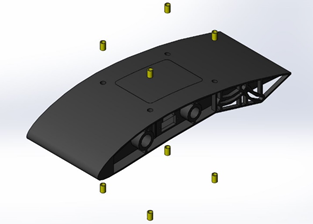
\includegraphics[width=\textwidth]{mid-span-rib}
        \caption{Mid-span}
        \label{fig:ribs:mid-span}
    \end{subfigure}
    \hfill
    \begin{subfigure}[b]{0.49\columnwidth}
        \centering
        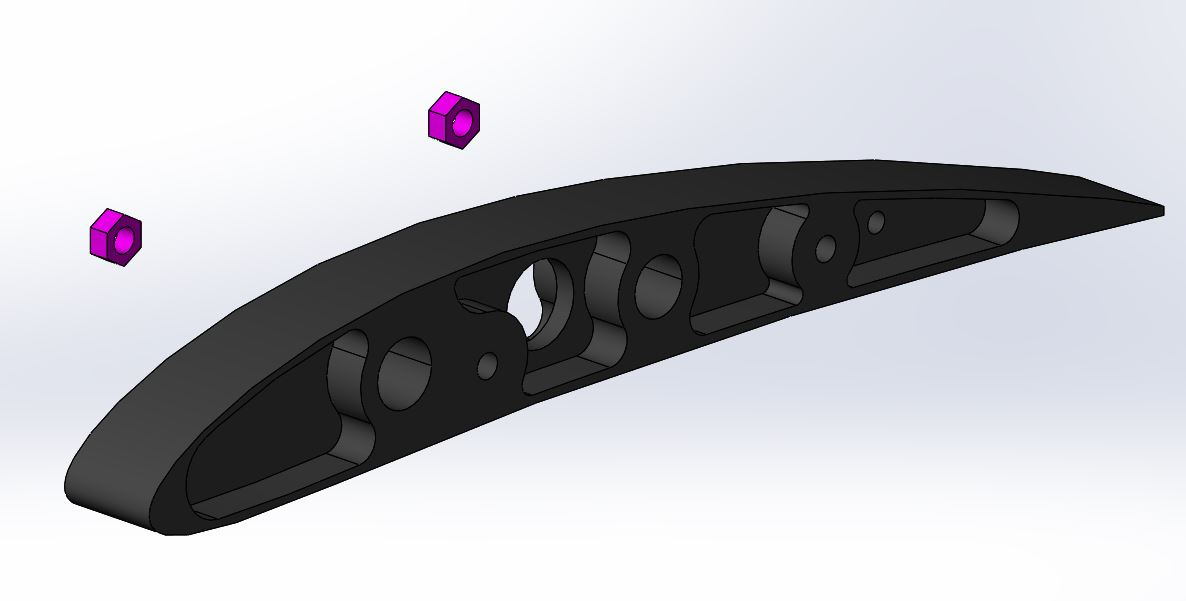
\includegraphics[width=\textwidth]{tip-rib}
        \caption{Tip}
        \label{fig:ribs:tip}
    \end{subfigure}
    
    \caption{CAD models of the wing ribs.}
    \label{fig:ribs}
\end{figure}

% \importimage{underwing-pusher}{underwing pusher configuration.}{Underwing pusher}{0.5}
% \importimage{underwing-tractor}{underwing tractor configuration.}{Underwing tractor}{0.5}
% \importimage{overwing-pusher}{overwing pusher configuration.}{Overwing pusher}{0.5}
% \importimage{overwing-tractor}{overwing tractor configuration.}{Overwing tractor}{0.5}
% \importimage{wingtip-pusher}{wingtip pusher configuration.}{Wingtip pusher}{0.5}
% \importimage{wingtip-tractor}{wingtip tractor configuration.}{Wingtip tractor}{0.5}

\begin{figure}[H]
    
    \centering
    \begin{subfigure}[b]{0.49\columnwidth}
        \centering
        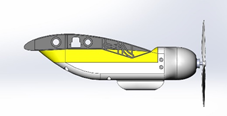
\includegraphics[width=\textwidth]{underwing-pusher}
        \caption{Underwing pusher}
        \label{fig:wing-mounting:underwing-pusher}
    \end{subfigure}
    \hfill
    \begin{subfigure}[b]{0.49\columnwidth}
        \centering
        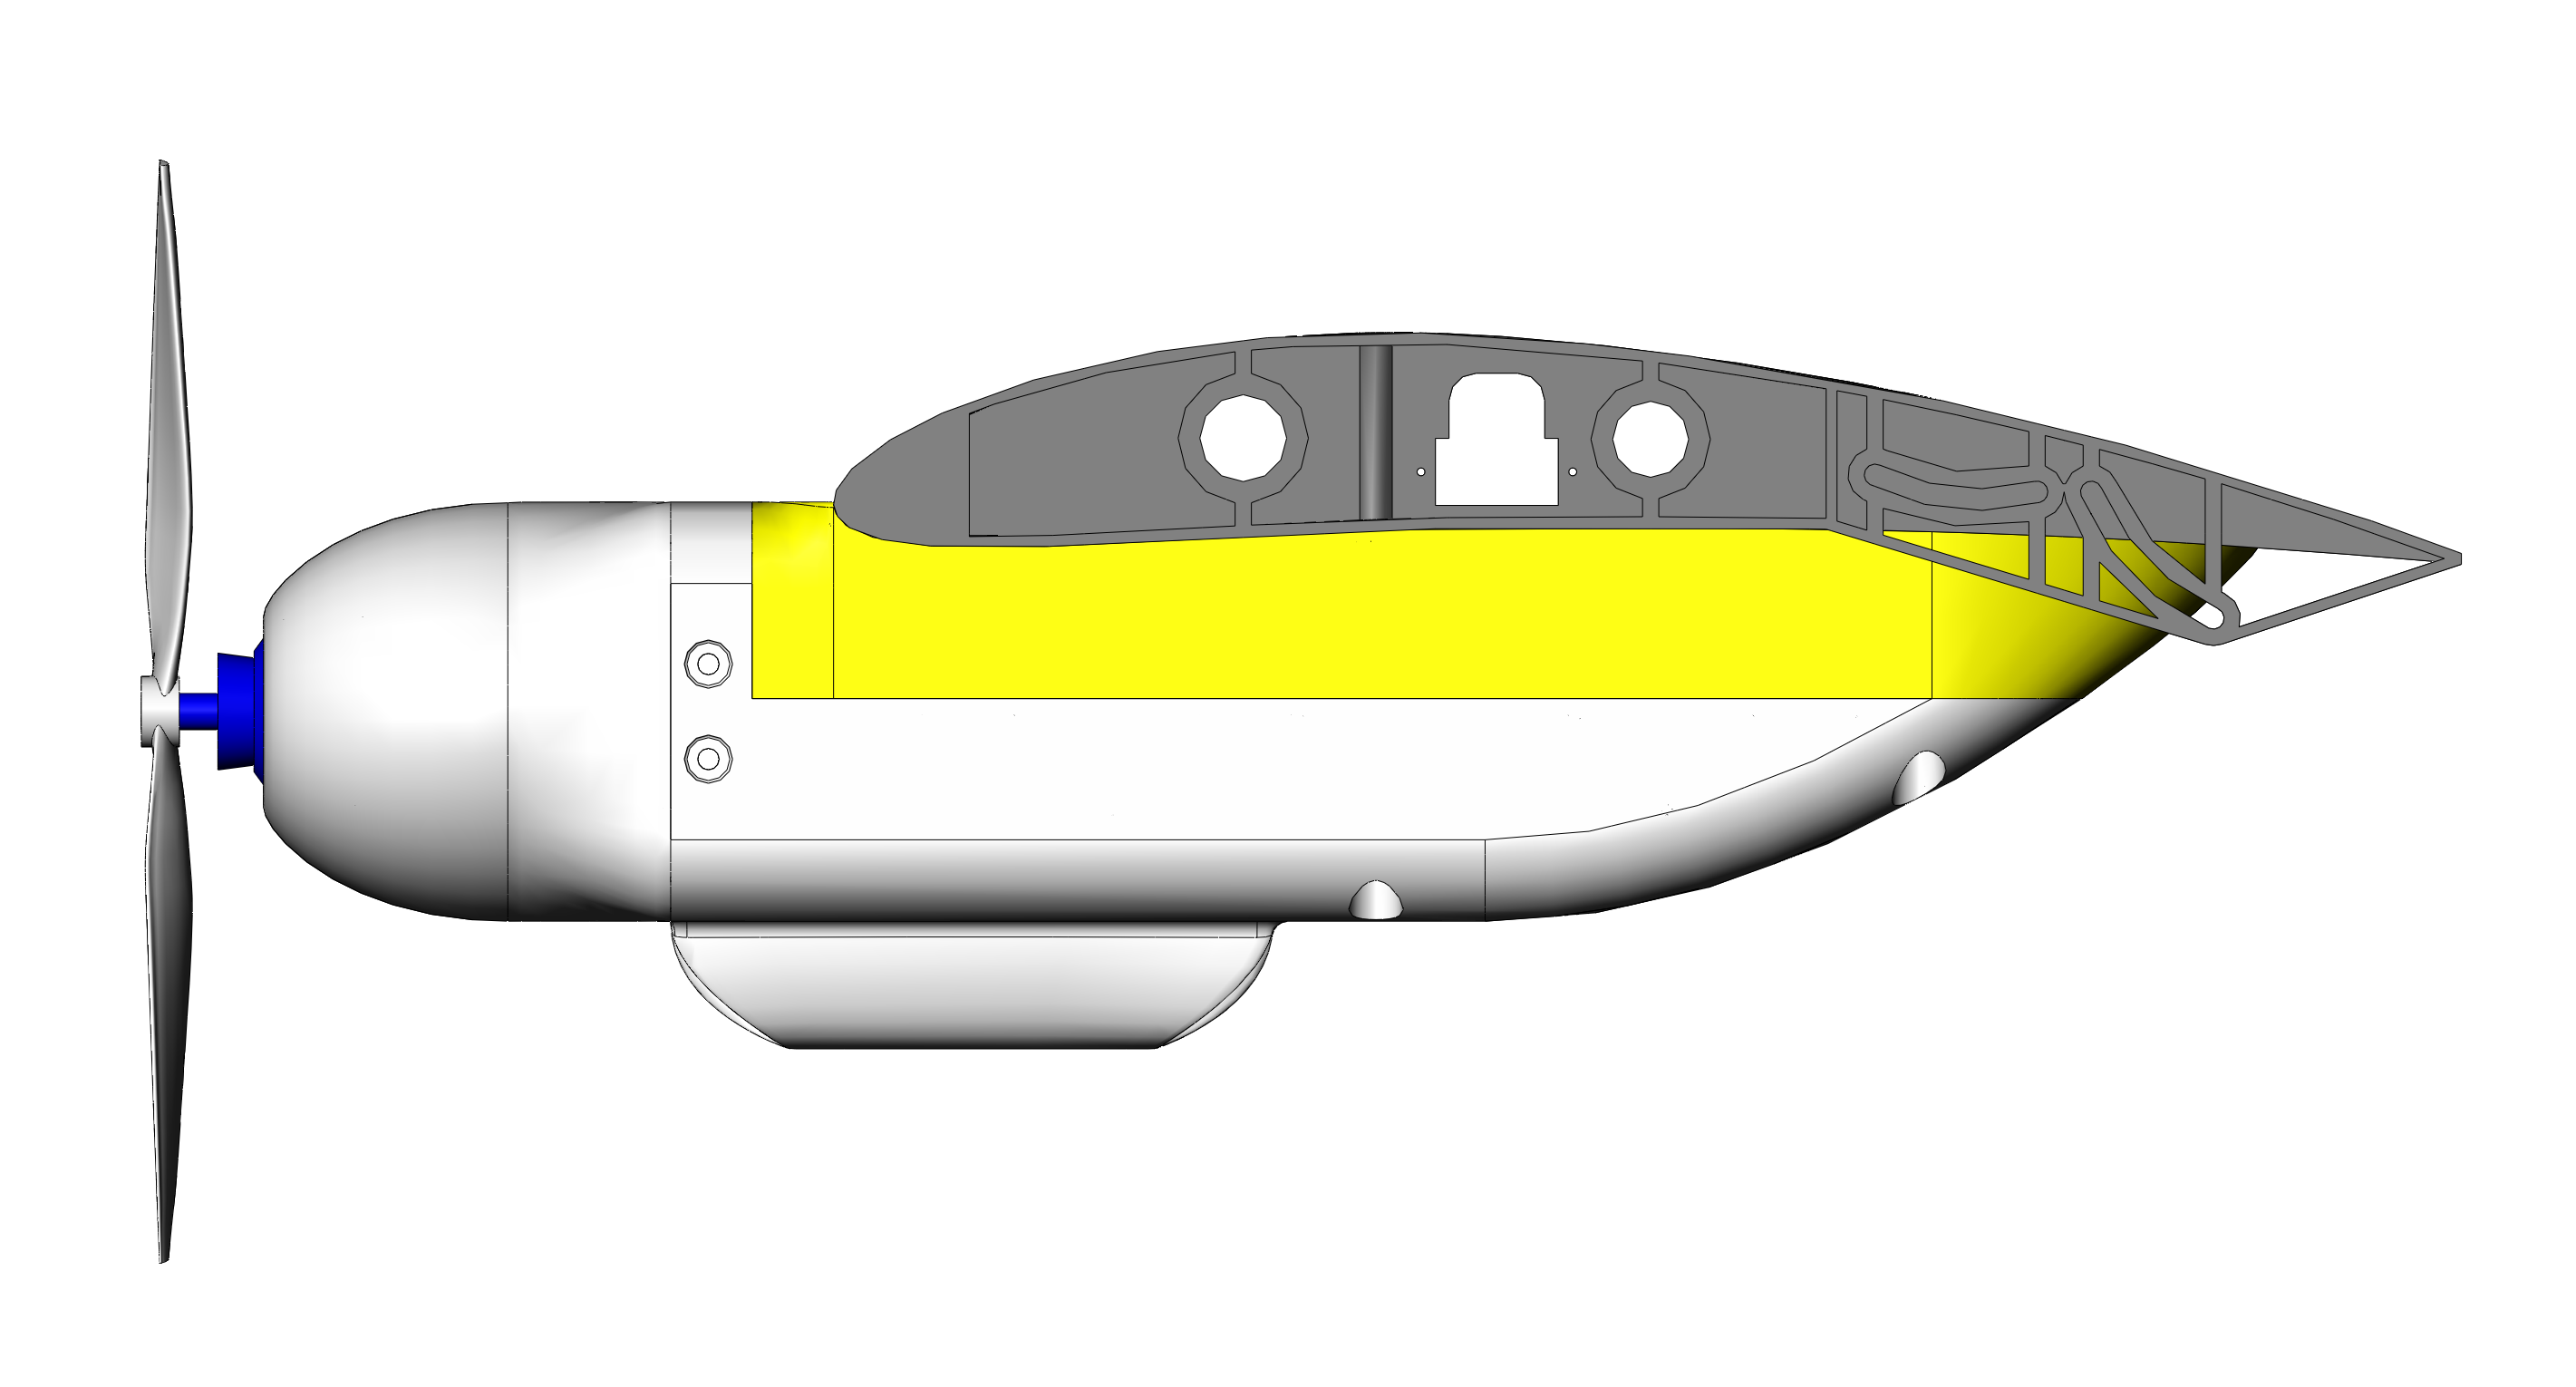
\includegraphics[width=\textwidth]{underwing-tractor}
        \caption{Underwing tractor}
        \label{fig:wing-mounting:underwing-tractor}
    \end{subfigure}
    
    \centering
    \begin{subfigure}[b]{0.49\columnwidth}
        \centering
        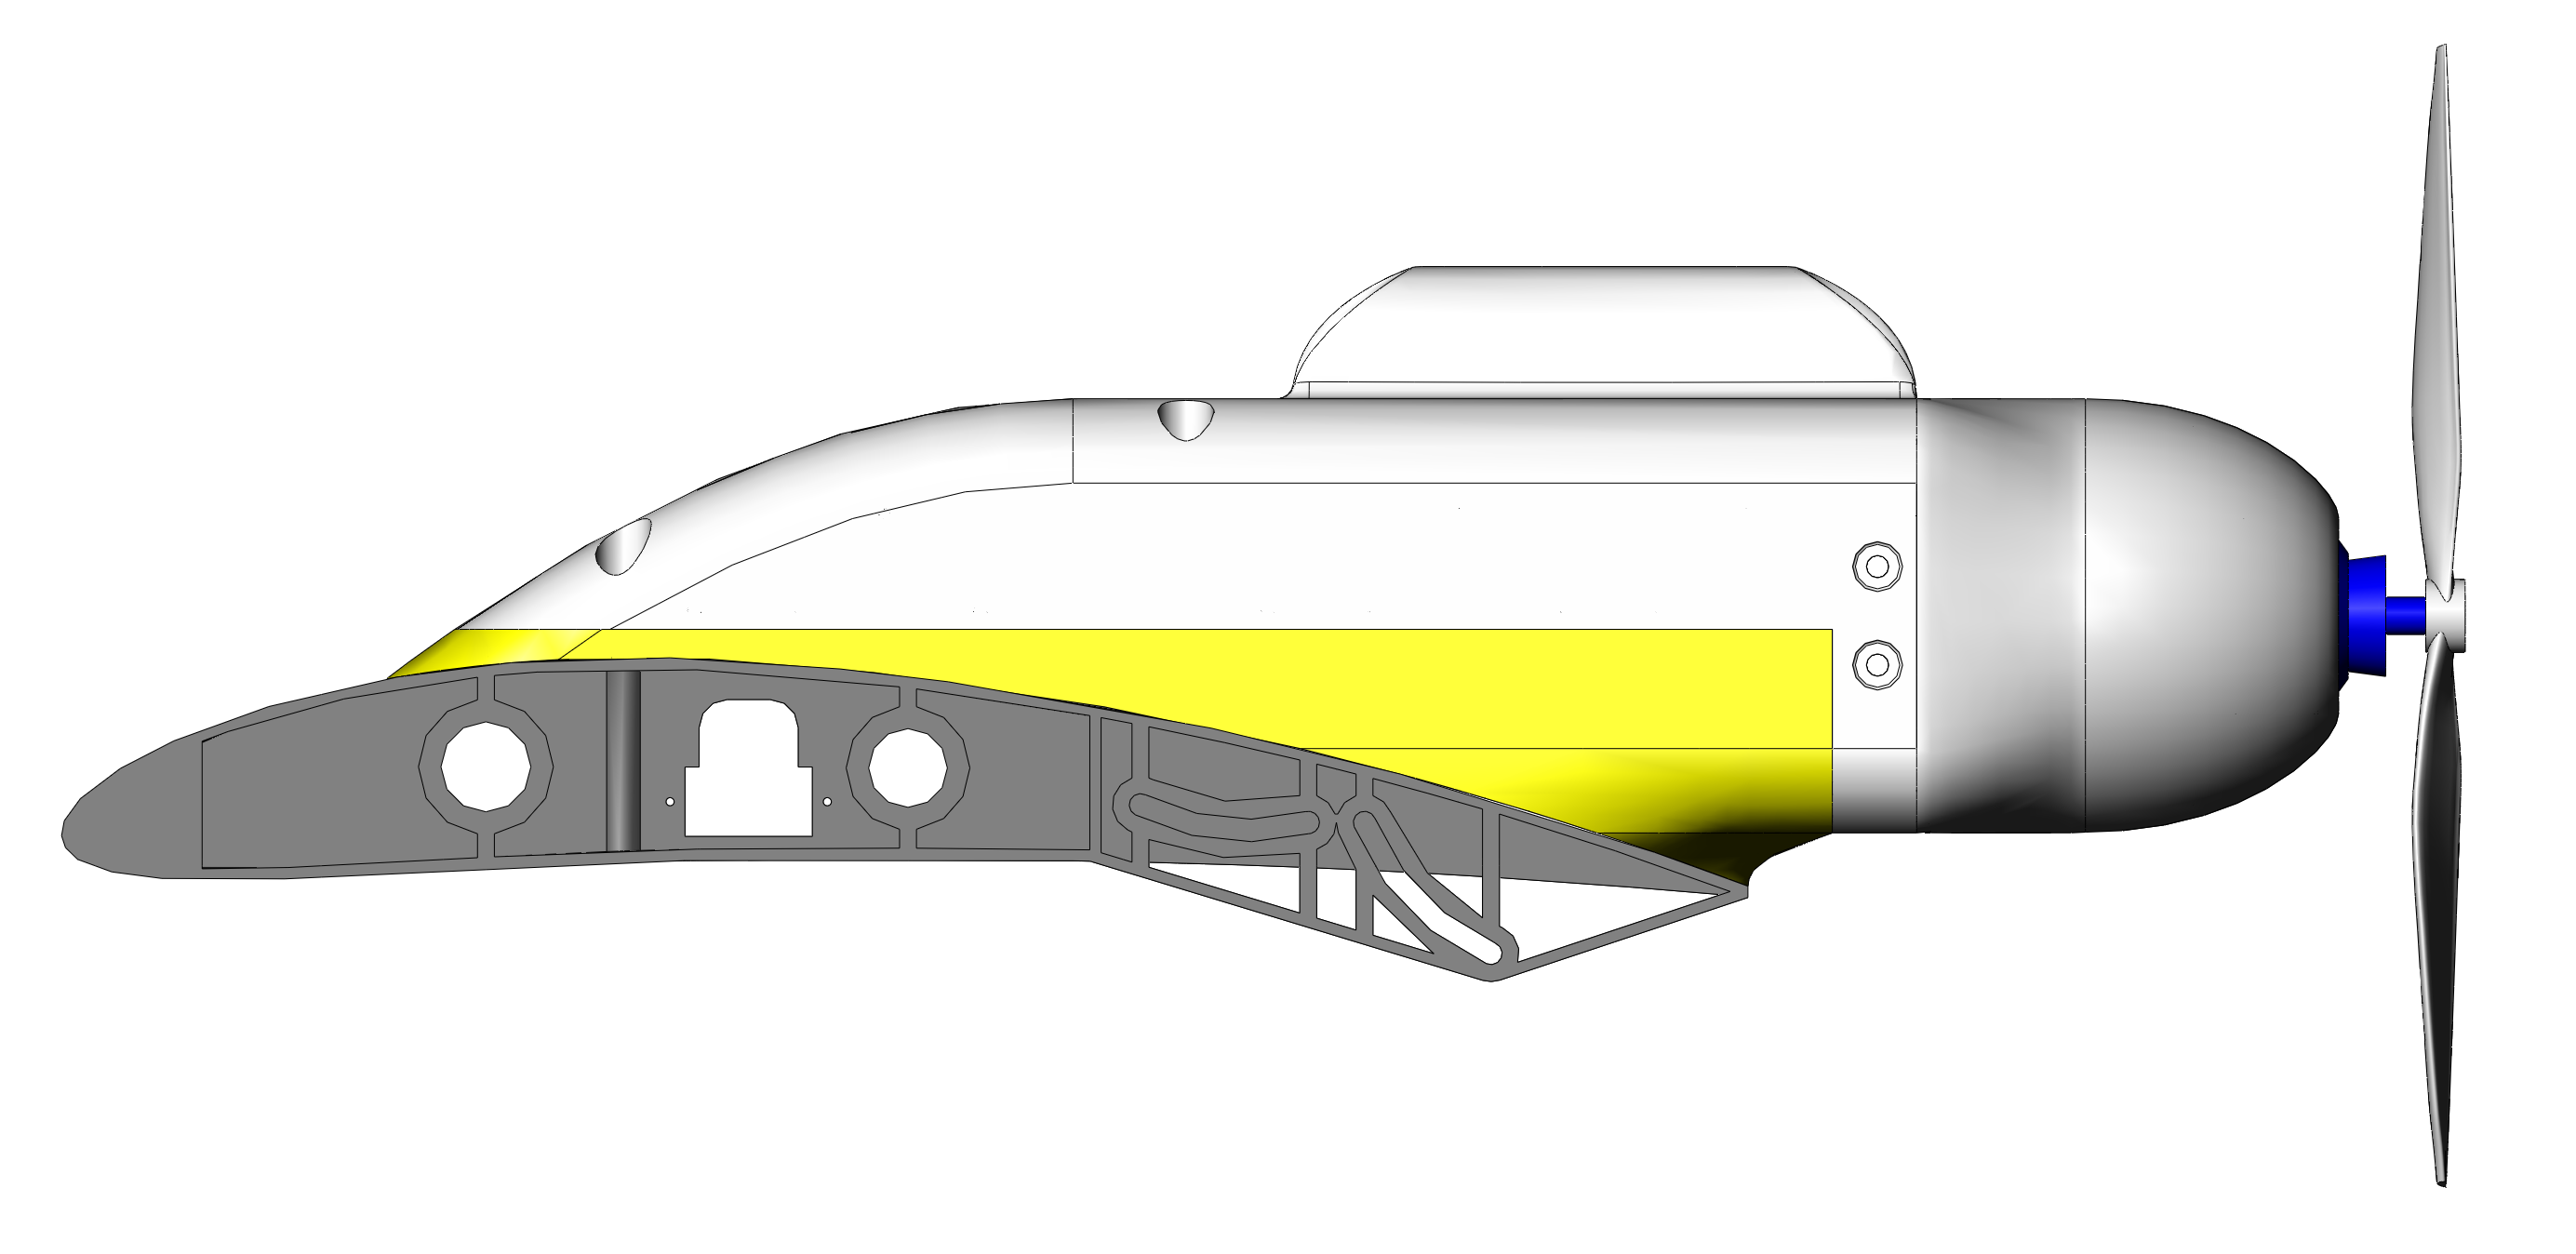
\includegraphics[width=\textwidth]{overwing-pusher}
        \caption{Overwing pusher}
        \label{fig:wing-mounting:overwing-pusher}
    \end{subfigure}
    \hfill
    \begin{subfigure}[b]{0.49\columnwidth}
        \centering
        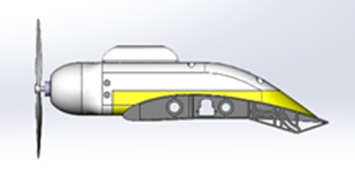
\includegraphics[width=\textwidth]{overwing-tractor}
        \caption{Overwing tractor}
        \label{fig:wing-mounting:overwing-tractor}
    \end{subfigure}
    
    \centering
    \begin{subfigure}[b]{0.49\columnwidth}
        \centering
        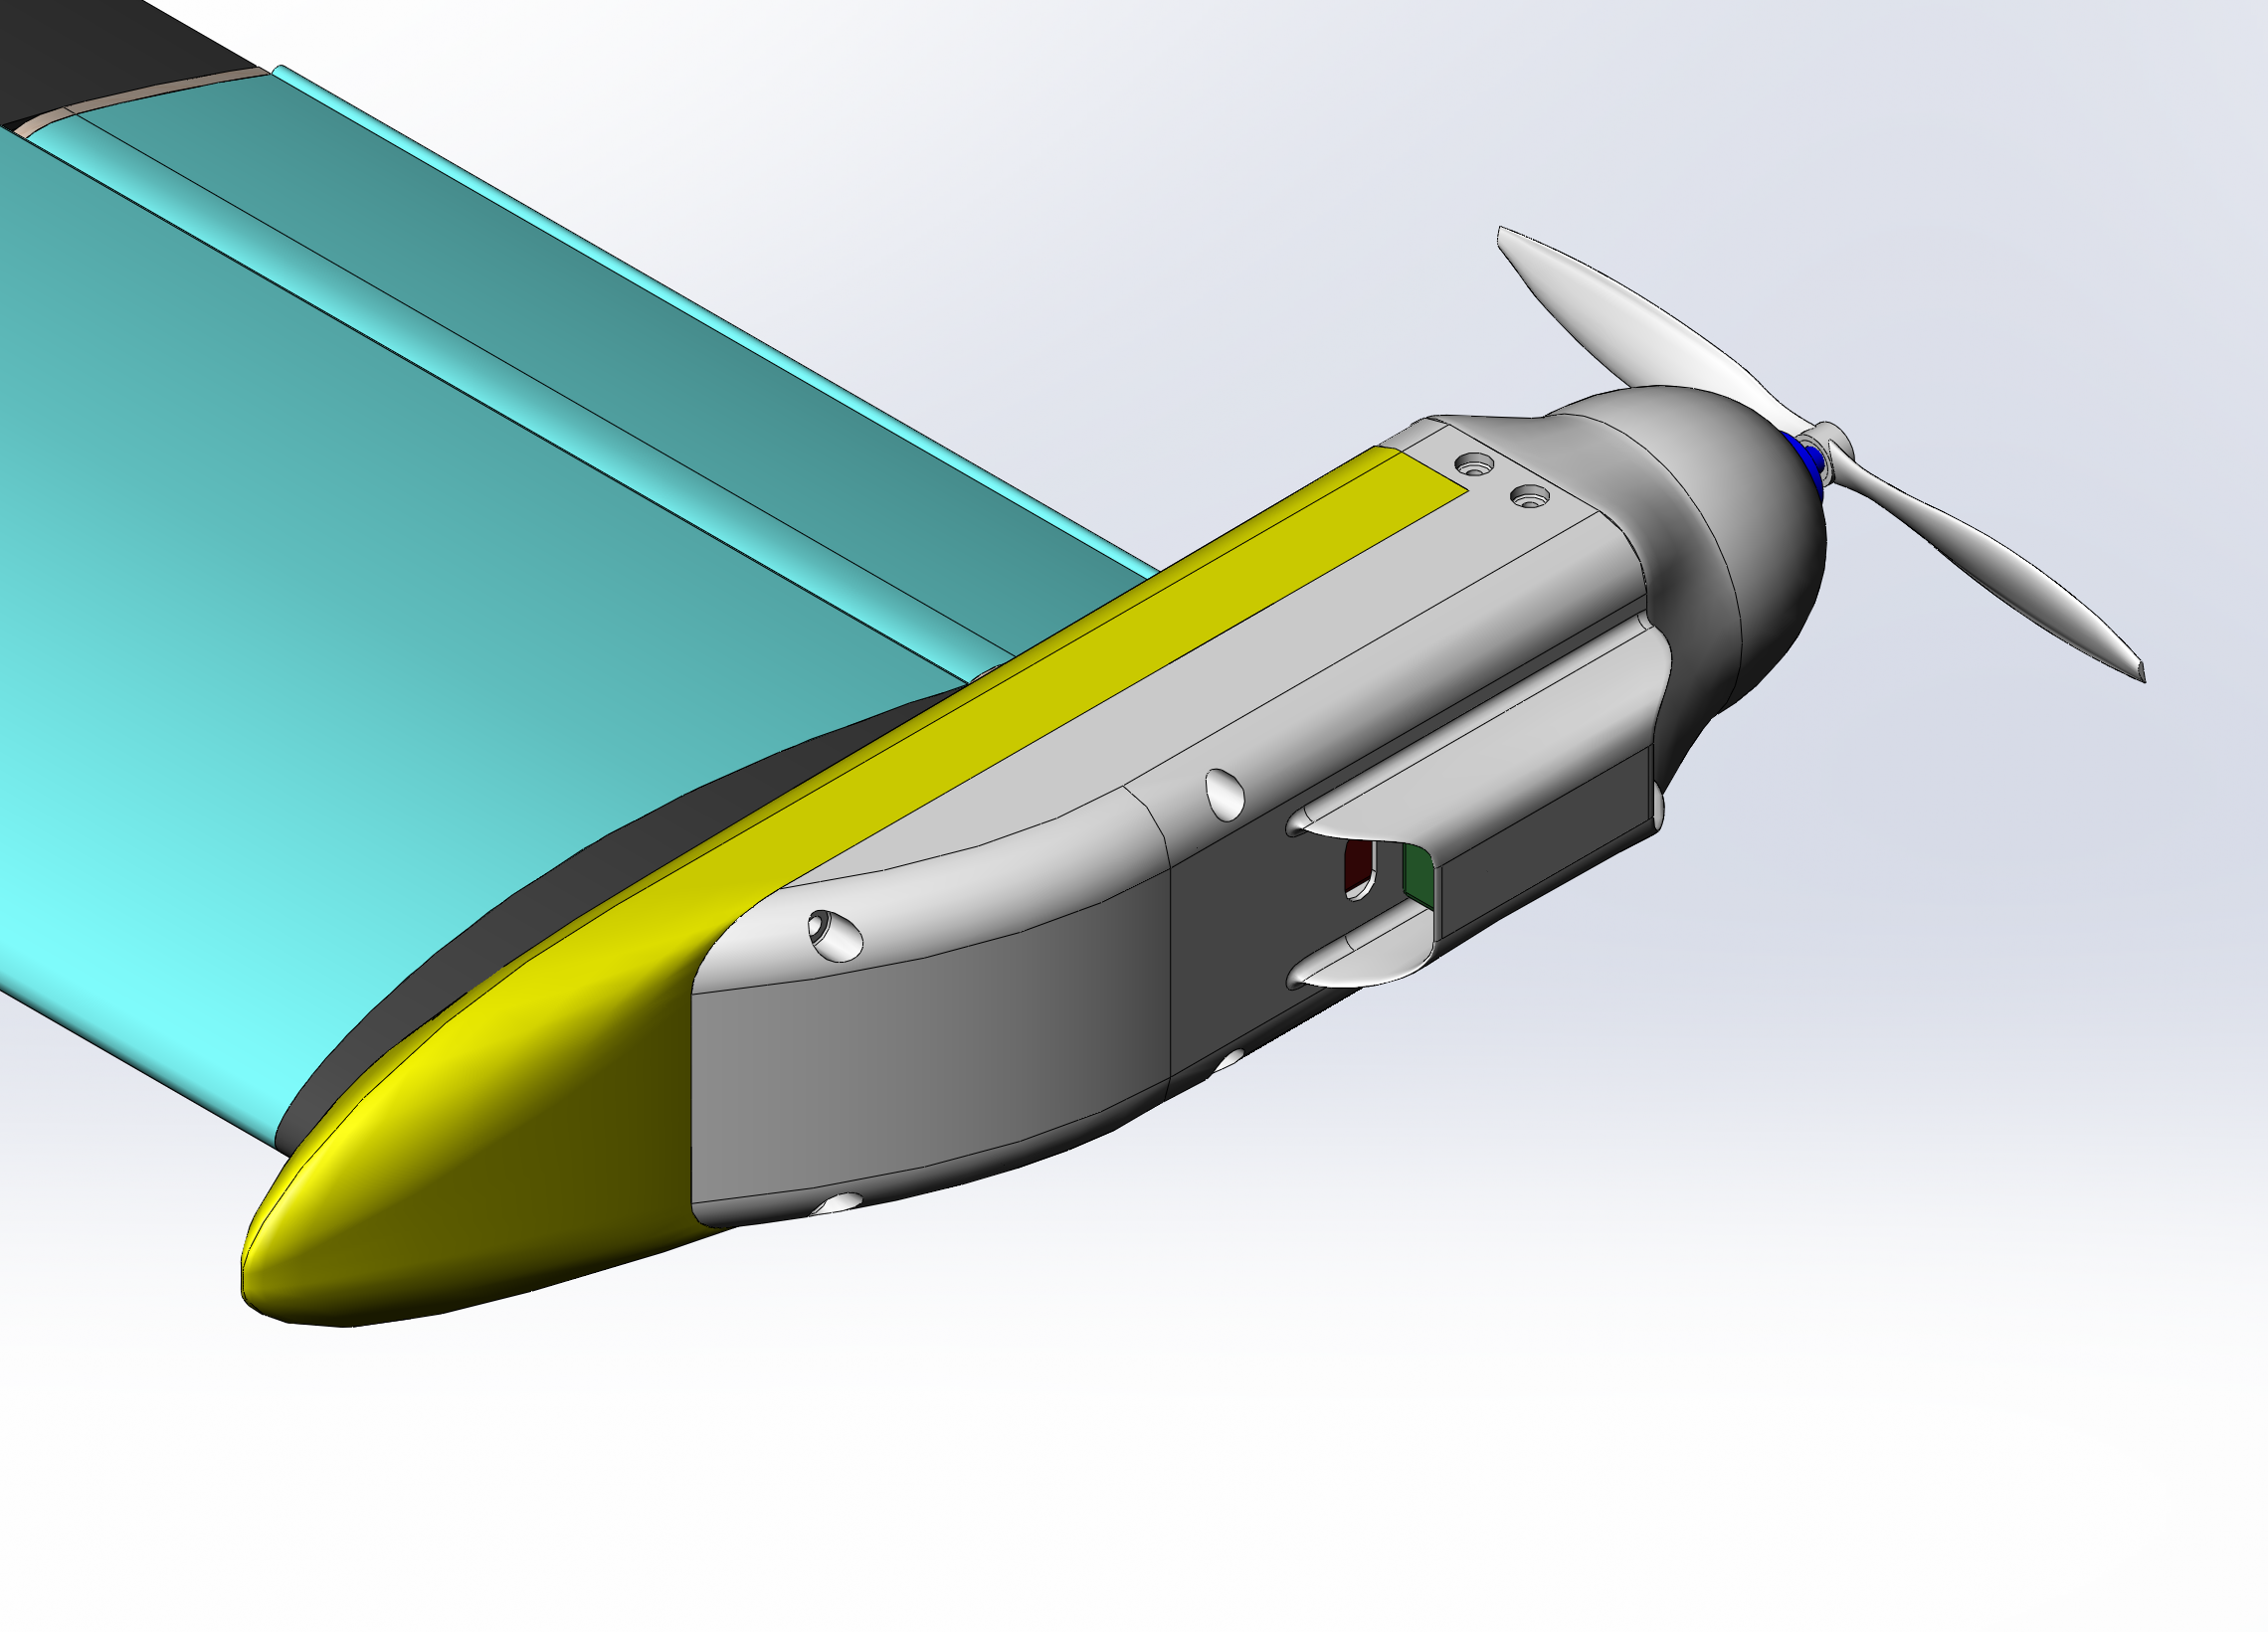
\includegraphics[width=\textwidth]{wingtip-pusher}
        \caption{Wingtip pusher}
        \label{fig:wing-mounting:wingtip-pusher}
    \end{subfigure}
    \hfill
    \begin{subfigure}[b]{0.49\columnwidth}
        \centering
        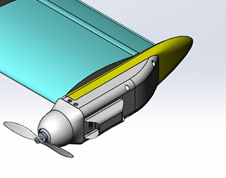
\includegraphics[width=\textwidth]{wingtip-tractor}
        \caption{Wingtip tractor}
        \label{fig:wing-mounting:wingtip-tractor}
    \end{subfigure}
    
    \caption{possible configurations of the PUC on the wing mounts.}
    \label{fig:wing-mounting}
\end{figure}

Each semi-span insert is equipped with four brass threaded inserts on both the top and bottom surfaces.
These permit the fastening of the power unit cells and the respective adapter.
The location of the holes is the same for top and bottom surface (when viewed from the top).
As such, the same motor housing can be mounted on the top and bottom surface without alterations.
Furthermore, as presented in Figure \ref{fig:wing-insert}, the inserts are equidistant from the centreline positioned at half chord, thereby allowing the mounting of the same power unit cell (PUC) in tractor or pusher configurations without the need for alterations. 

\importimage{wing-insert}{section view of the wing insert.}{Wing insert}{0.9}

The tip insert is designed to mount the motor housing in a horizontal orientation.
In order to use the same configuration of mounting points the tip adaptor covers a structural role, unlike the others.
This presents the brass inserts configuration discussed above so to guarantee the attachment of the standardized PUC.  % TODO: clarify meaning
The adapter is then mounted to the insert though two M6 bolts fastened to the two imbedded nuts shown in Figure \ref{fig:ribs:tip}. 

In order to reduce the number of elements comprising the wing assembly, these components cover the function of ribs as well providing further torsional rigidity to the wing structure.
The two holes shown in Figure \ref{fig:wing-insert} permit the carbon spars to run through the rib insert, providing a secure attachment and sufficient bonding area.
Furthermore, as will be discussed in more detail later, the housing for the active surfaces' servos and flap guides are designed to be an integral part of the rib structure. 

\subsection{Mounting plate} \label{sec:final-design-proposal:wing:mounting-plate}

A nylon printed mounting plate is located at the centre of the wing assembly and is tightly mounted to the wing spars so as to guarantee a rigid support.
The wing assembly is then clamped onto the fuselage attachment plate by four M6 bolts.
These are positioned at the corners of the 3D printed plate as shown in Figure \ref{fig:wing-assembly}.
A styrofoam cover placed on top of the mounting plate is responsible for the blending of the wing assembly with the rest of the fuselage. 

\importimage{wing-assembly}{exploded view of the wing assembly attachment procedure}{Wing assembly attachment}{0.8}

The two cylinders housing the carbon spars (Figure \ref{fig:wing-plate:cad}) ensure an even distribution of the loads though a large area.
This is essential since this component is subject to the entirety of the load transferring from the wing to the fuselage and vice versa.
Extensive work was therefore conducted using finite element analysis to generate a reliable and light design.
The peak loading for this component was established to be $4g$, simulating an abrupt increase in lift as in Figure \ref{fig:wing-plate:fea}, and producing the optimal design that was eventually used. 

% \importimage{wing-plate-cad}{CAD representation of the wing mounting plate.}{Wing mounting plate CAD}{0.6}
% \importimage{wing-plate-fea}{stress concentration due to an applied load of 275 N.}{Wing mounting plate FEA}{0.6}

\begin{figure}[H]

    \centering
    \begin{subfigure}[b]{0.49\columnwidth}
        \centering
        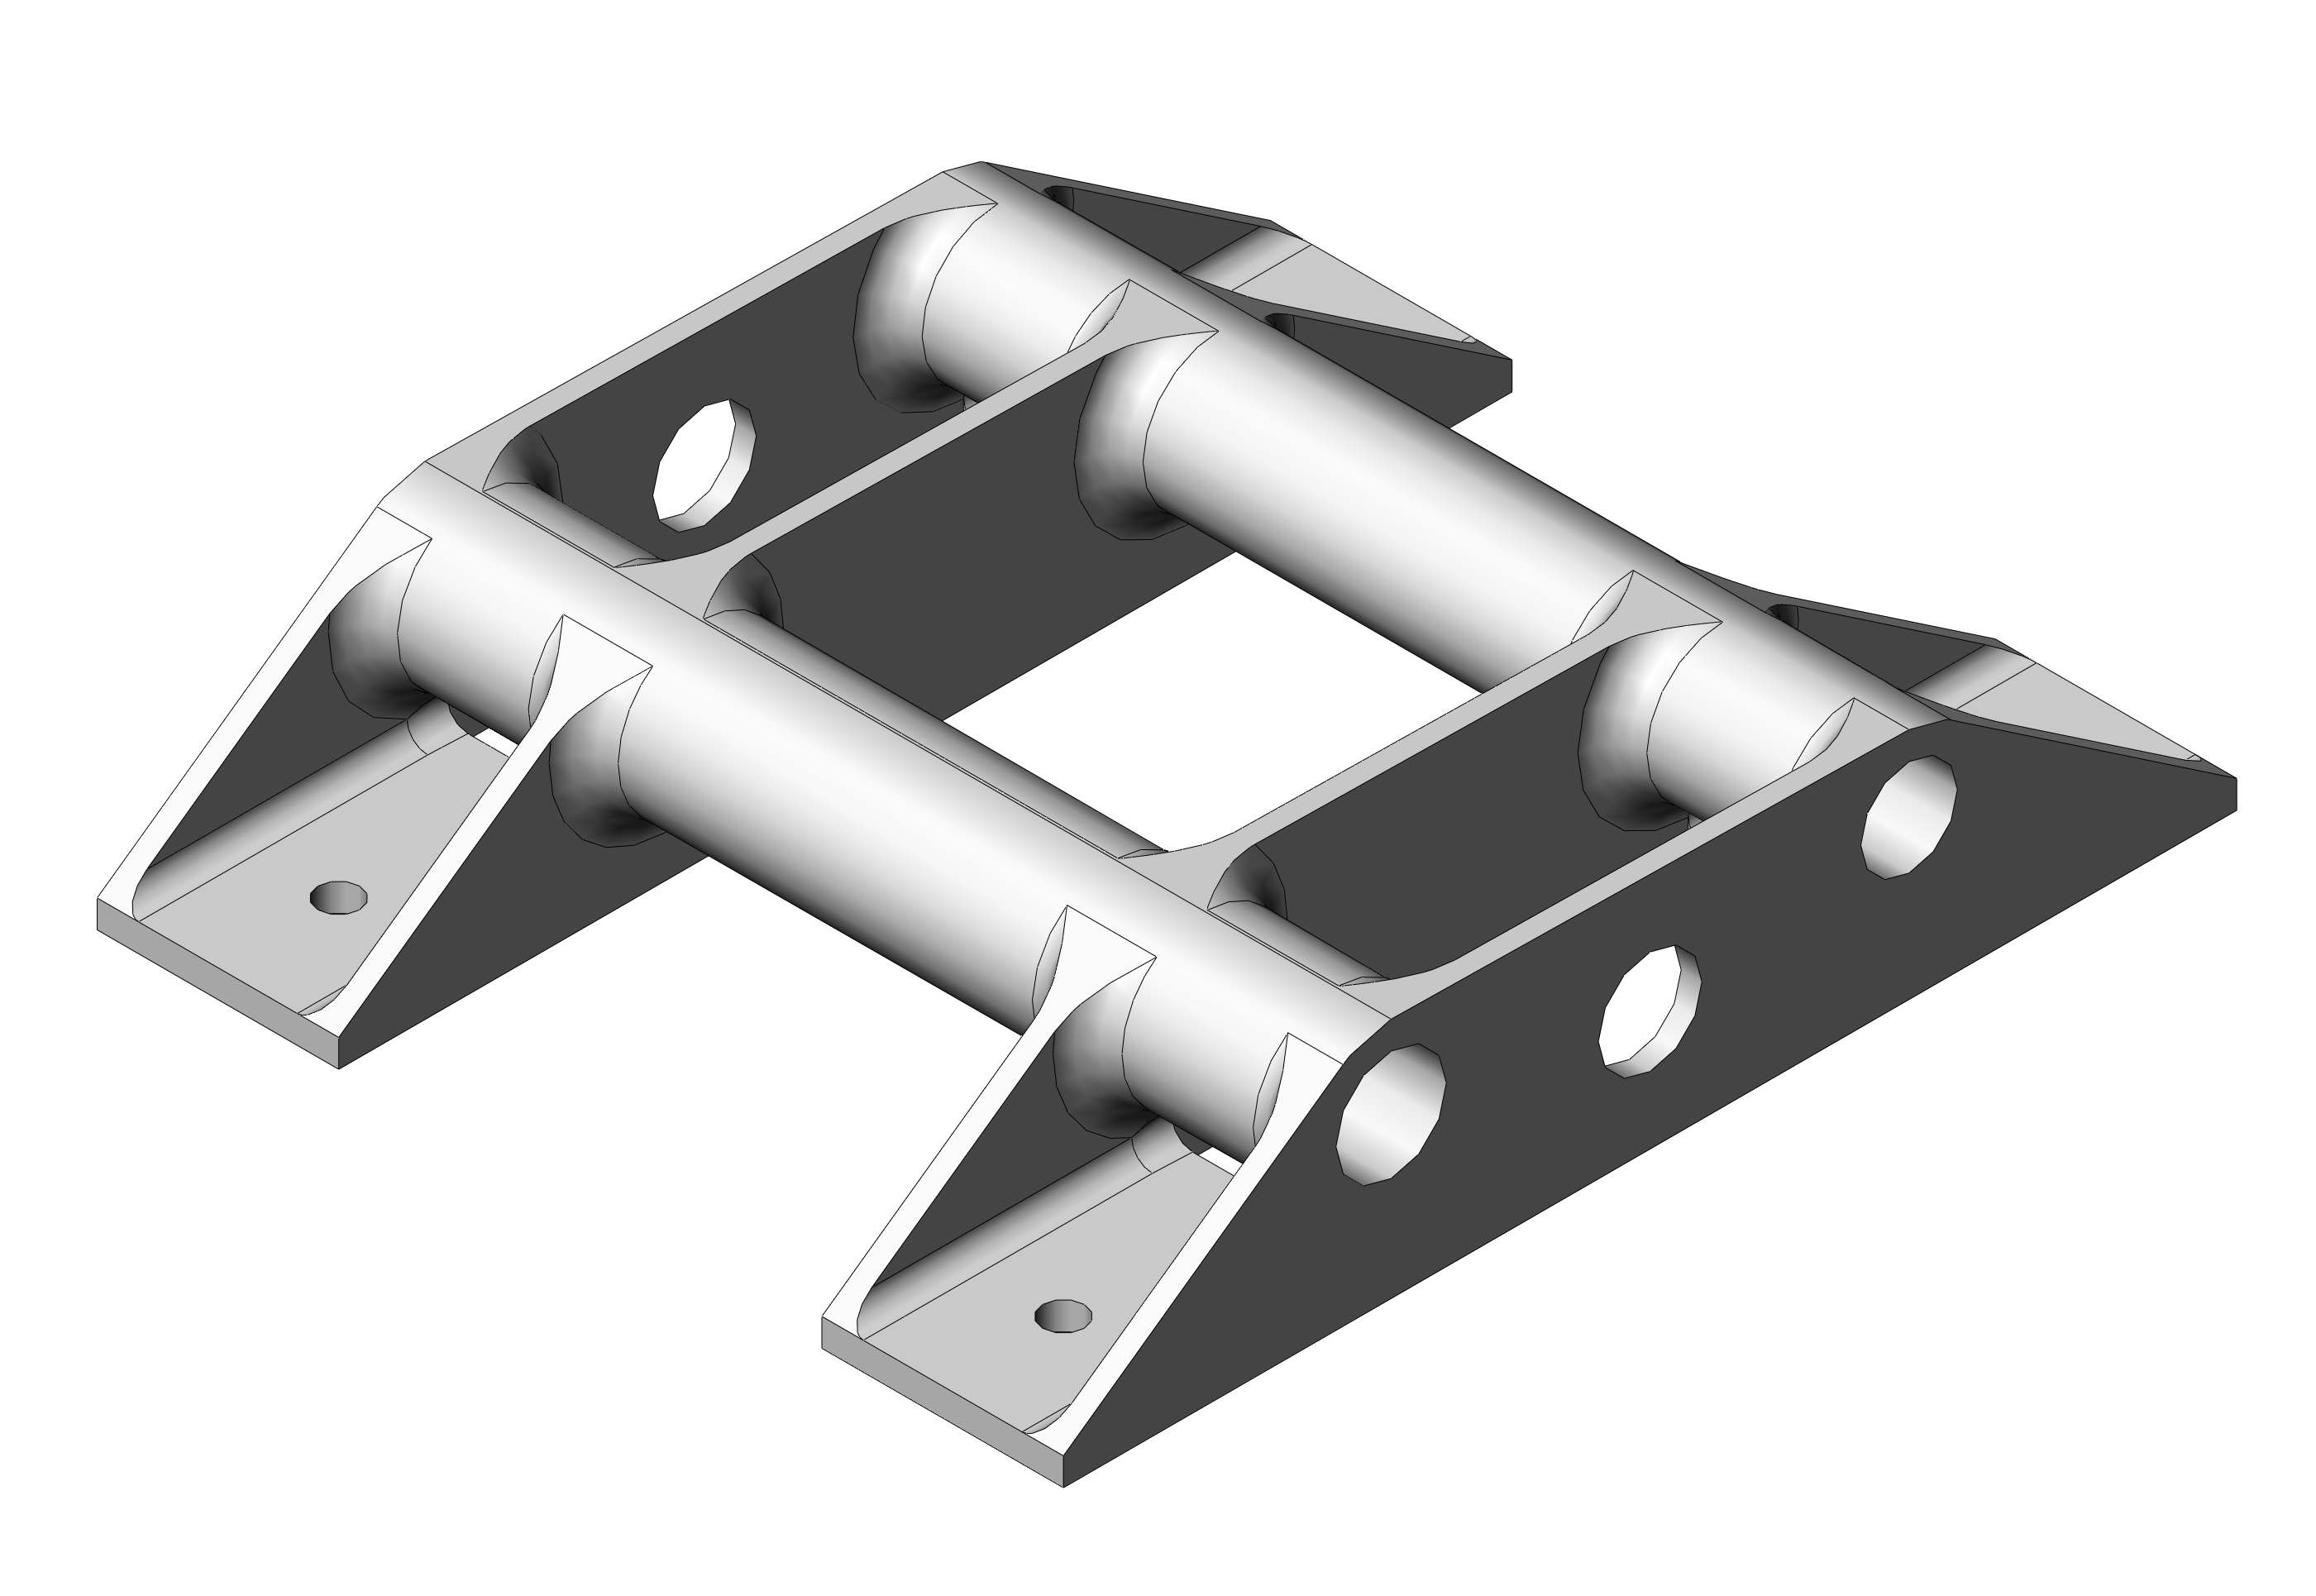
\includegraphics[width=\textwidth]{wing-plate-cad}
        \caption{CAD}
        \label{fig:wing-plate:cad}
    \end{subfigure}
    \hfill
    \begin{subfigure}[b]{0.49\columnwidth}
        \centering
        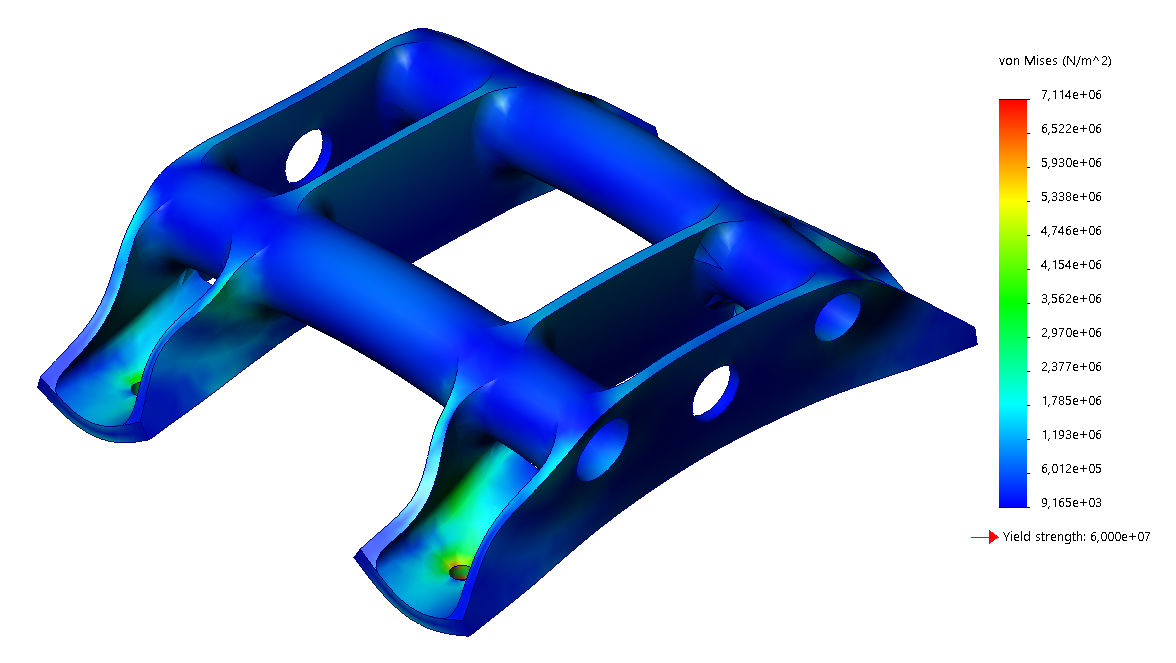
\includegraphics[width=\textwidth]{wing-plate-fea}
        \caption{FEA}
        \label{fig:wing-plate:fea}
    \end{subfigure}
    
    \caption{
        models of the wing mounting plate; (b) shows the stress concentration under a \newtons{275} load.
    }
    \label{fig:wing-plate}
\end{figure}

\section{Landing gear} \label{sec:final-design-proposal:landing-gear}

Using a similar process to that used in the original tail wheel design, it was calculated that the main landing gear would experience up to \newtons{105.8} on landing.  % TODO: add section reference if reordered
The main gear in the final design proposal is located behind the centre of gravity, behind the internal electronics.
This, along with a redesigned fuselage means the landing gear could be designed as a single part and attached easily to the bottom of the fuselage. 

% \importimage{main-gear-design}{main gear design.}{Main gear design}{0.4}
\importimage{main-gear-fea}{main gear FEA stress results.}{Main gear FEA}{0.6}

The main shape of the design remains unchanged from the initial design, and is a similar design to that seen on many small UAVs which is simple, easy to implement, and robust.
The final design is expected to experience a maximum stress of 92.5 MPa on a rough landing, and is manufactured from carbon fibre because it can be manufactured cheaply in university workshops and has a high strength to weight ratio.
The final design has a maximum thickness of \mm{6} at the top where it joins the fuselage, narrowing to \mm{4} by the wheels.
The depth remained constant at \mm{65}, with a wheelbase of \mm{490} and a height of \mm{220} to avoid hitting the under-rudder on takeoff.
The redesigned fuselage structure with two lower plates means that the landing gear can easily be mounted to the fuselage using two M4 bolts. 

Eventually, a landing gear model very similar to the one described here was found online and purchased instead of manufacturing one from scratch; this was found to be more time- and cost-effective.

\importimage{landing-gear-join}{landing gear joining mechanism.}{Landing gear joining mechanism}{0.6}

The nose gear was chosen at the recommendation of the project co-supervisor and is the same as the one used on the SPOTTER aircraft \cite{spotter-19}, a \kg{24} split fuselage UAV.
It is easy to implement into the nose and is steerable, while also being cheap, lightweight, and strong. 

\section{Nose} \label{sec:final-design-proposal:nose}

The final design of the nose incorporates a steerable landing gear.
This part of the design was carefully considered throughout the design process, but only fully implemented after the landing gear design had been finalised. 

% \importimage{steerable-gear}{integration of the steerable nose gear.}{Steerable nose gear}{0.7}

Figure \ref{fig:nose-design:steerable-nose-gear} shows how the nose gear is incorporated within the vent design.
The nose gear is secured using two collars, one above and one below the thicker part of the nose, as well as one to secure the servo arm in place.
The servo arm is attached to the servo via two springs, which alleviate impacts and prevent the nose from rapid direction changes due to bumps.
The servo is bolted onto the battery tray, to one side, to allow space for the battery tray to be removed. 

As mentioned during the analysis of the landing gear, depending on the configuration, the landing gear will have to withstand a force of up to around \newtons{35} on landing.
Therefore, further FEA was carried out on the nose.
The results (Figure \ref{fig:nose-connection-fea}) show a moderate level of stress on the wall at the bottom of the vent, although this was about half of the perceived yield strength of the SLS nylon which is to be used. 

\importimage{nose-connection-fea}{FEA on nose and landing gear connection.}{Nose connection FEA}{0.7}

When the nose motor is not needed it can be removed and replaced with a small insert.
The hollow insert is to be 3D printed on the university 3D printer using PLA as it is not a structural component.
It was designed to be screwed in in the same manner as the motor. 

\importimage{nose-motor-filler}{nose motor filler.}{Nose motor filler}{0.5}

\section{Fuselage} \label{sec:final-design-proposal:fuselage}

\subsection{Central structure} \label{sec:final-design-proposal:fuselage:central-structure}

The main focus for the design of the UAV's fuselage was to provide a reliable and simple platform for the experiments.
The concept for the design of the fuselage revolved around the idea of providing easy access to the electronics.
Changing the motor configuration multiple times demands the ability to check and modify the electronics with ease in order to proceed with the experiments in a smooth manner.
The design therefore presents a large electronics tray placed in the lower section of the fuselage, shown in purple in Figure \ref{fig:fuselage-inner-structure}.
This can be accessed through the removal of the UAV's nose.

\importimage{fuselage-inner-structure}{CAD representation of the inner structure of the fuselage's central section.}{Fuselage inner structure}{0.8}

All of the fuselage's structural components are located in the top section of this part.
In so doing a large area was created for the housing of the electronics as shown in Figure \ref{fig:fuselage-inner-structure}.
The supports for the electronics tray, also referred as the fuselage ribs, were designed to be manufactured out of \mm{5} birch wood sheets.
Such supports (shown in brown in Figure \ref{fig:fuselage-inner-structure}) are mounted onto the fuselage central beam.
This is a square section carbon spar (\mm{20} $\times$ \mm{20}) which extends for the entire fuselage length. 

A carbon fibre sandwich panel is placed onto the top surface of the fuselage's central spar.
This is bonded at the wing's attachment area with the aid of epoxy bonding agent.
Its function is to provide the four mounting points for the bolts so as to allow the fixing of the wing assembly to the fuselage.
The sandwich panel is comprised of a \mm{5} thick nomex core placed between two carbon skins.
These are each made out of three ply woven carbon prepreg cured in autoclave.
Mounted below the plate are two PLA printed brackets (Figure \ref{fig:pla-bracket}); these are responsible for the correct positioning of the fuselage ribs and the landing gear mounting structure (Figure \ref{fig:brackets-highlighted}).
Furthermore, they are designed to withstand a vertical load of \newtons{170} each, thus offering a redundant attachment for the mounting plate in case of failure.

\importimage{pla-bracket}{CAD representation of the PLA bracket.}{PLA bracket}{0.5}
\importimage{brackets-highlighted}{fuselage central assembly with brackets highlighted in green.}{Highlighted brackets}{0.7}

\subsection{Landing gear attachment} \label{sec:final-design-proposal:fuselage:landing-gear-attachment}

The aircraft was designed to not exceed \kg{7} of total mass.
Hence the position and the mass of the landing gear structure proved to be of significance in positioning the aircraft's centre of gravity.
Its ideal position was set to be at \pc{50} of the wing's chord length, with a \pc{5} shift caused by the change in propulsion configuration.
The landing gear is mounted on two C-shaped \mm{5} aluminium brackets.
These are mounted to two bulkheads as shown in Figure \ref{fig:landing-gear-attachment}, and fulfil the role of transferring and absorbing the vertical loads encountered during taxi, takeoff, and landing.
In order to minimise the weight of this structure the bulkheads were designed to be manufactured as carbon fibre sandwich panels.
These have been specified to withstand vertical loads up to $5g$.
Furthermore, two triangular braces, as shown in Figure \ref{fig:landing-gear-attachment:side}, are attached to the lowest section of the bulkheads and are clamped to the main spar through a PLA insert.
These work in compression and are designed to counteract the moments generated by the loads acting on the wheels in the direction of travel. 

% \importimage{landing-gear-attachment}{landing gear attachment structure.}{Landing gear attachment}{0.4}
% \importimage{landing-gear-side}{landing gear attachment side view.}{Landing gear attachment side view}{0.4}

\begin{figure}[H]

    \centering
    \begin{subfigure}[b]{0.4\columnwidth}
        \centering
        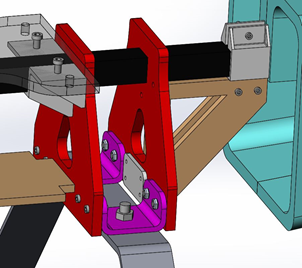
\includegraphics[width=\textwidth]{landing-gear-attachment}
        \caption{}
        \label{fig:landing-gear-attachment:angled}
    \end{subfigure}
    \hfill
    \begin{subfigure}[b]{0.49\columnwidth}
        \centering
        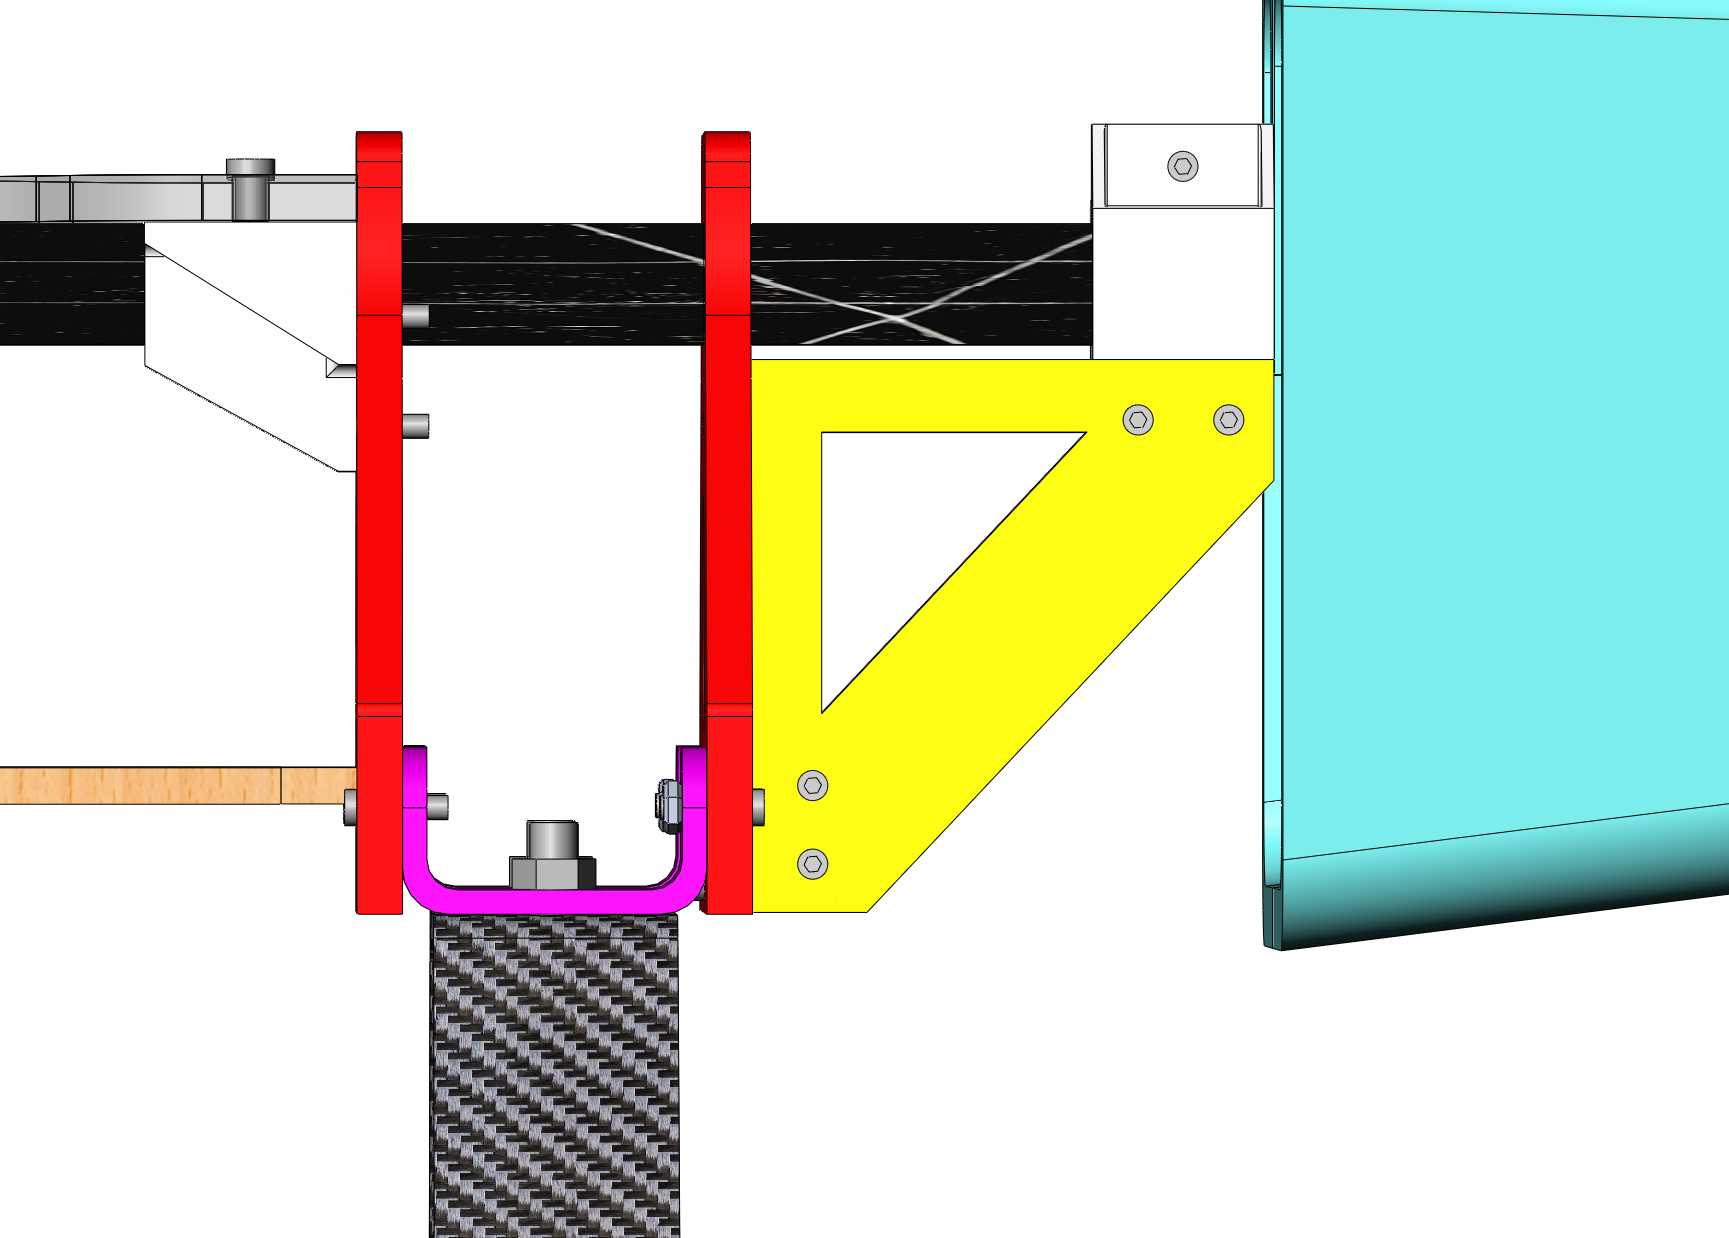
\includegraphics[width=\textwidth]{landing-gear-side}
        \caption{}
        \label{fig:landing-gear-attachment:side}
    \end{subfigure}
    
    \caption{landing gear attachment structure.}
    \label{fig:landing-gear-attachment}
\end{figure}

The carbon fibre sandwich panels bulkheads were designed in the same manner as the aforementioned fuselage central plate, whose schematic can be seen in Figure \ref{fig:carbon-fibre-sandwich}. 

\importimage{carbon-fibre-sandwich}{CAD representation of the carbon fibre sandwich panel components.}{Carbon fibre sandwich}{0.5}

\subsection{Fuselage Structural Analysis} \label{sec:final-design-proposal:fuselage:finite-element-analysis}

In order to verify the strength of the design and identify any weak points, some FEA was carried out using the simulation function in SolidWorks.
This is a fairly basic FEA system and can only use coarse meshes $-$ otherwise the simulations fail due to too many cells $-$ but it gives a good indication of the strong and weak areas of the fuselage design.
The materials of the parts of the fuselage were all specified and the data for those materials applied as accurately as possible in order to ensure the parts' relative strengths were reflected in the simulations.
The model was stripped down to the minimum components required to perform the simulations in order to save computational time and simplify the simulations.
Initially a simulation was run to test the effects of high turning loads, with the main tail boom fixed in place as the reference point of the study, with loads of \newtons{210} applied vertically upwards on the wing spar holes in the wing mount, and \newtons{80} applied vertically down on the component tray, with the loads experienced by the nose and tail neglected for simplicity to focus purely on the central fuselage section.
These loads were chosen to simulate $3g$ loads in a turn, with the mass of the components assumed to be evenly distributed over the tray.
Figure \ref{fig:fuselage-stress-distribution} shows the results.

\importimage{fuselage-stress-distribution}{fuselage stress distribution during a simulated $3g$ turn.}{Fuselage stress distribution}{0.7}

It can be seen that the wing mount shows that the maximum stress experienced is around 1.6 MPa, which is significantly below the 30 MPa yield stress of the ABS material used.
The other high stress locations are on the lower parts of the component tray mounts, which peak at over 2 MPa, but the plywood used has a yield stress of 30 MPa and so this is also well below the point of breaking.
It can also be seen that the stress on the carbon fibre tail boom reaches over 2 MPa, but this is well below the yield stress of the carbon tube which will be over 600 MPa based on the properties quoted at \cite{unknown}. % TODO: [Performance Composites [REF]]. 

The second simulation determined the effects of landing loads, with the tail boom again fixed and the loads applied at the locations of the wheel centres on the landing gear.
This simulation only tested the main gear as this is where the highest forces should be experienced if the UAV is landed properly.
The forces applied are \newtons{350} vertically up and \newtons{105} horizontally backwards to simulate a heavy landing of $5g$ with $1.5g$ deceleration force. 

\importimage{landing-leg-simulation}{simulated stress distribution over one of the landing legs.}{Landing leg simulation}{0.4}
\importimage{fuselage-landing-simulation}{stress distribution over the fuselage during a simulated landing.}{Fuselage landing simulation}{0.6}

It can be seen in Figure \ref{fig:landing-leg-simulaion} that the peak loads experienced by the landing gear are around 260 MPa, which is below the yield stress of the carbon fibre as previously stated, and although it is nearing the yield stress, this is an extreme case of a particularly heavy landing and so a heavier landing than this would not be expected unless it occurs in a crash landing scenario (in which case the UAV's survival can never be guaranteed).
It can also be seen that the peak stress on the landing gear brackets is around 100 MPa, below the yield stress of around 270 MPa of the aluminium from which they are made.
With the scale modified to a reduced upper bound, the stresses on the other parts can be seen, with the peak stress experienced by the landing gear mounts seen as around 10 MPa, which is 50x below the yield stress of carbon fibre and so $-$ although the properties of carbon fibre sandwich panel are varied $-$ this is not close to failure. 

<<<<<<< HEAD
=======
\section{Landing gear} \label{sec:final-design-proposal:landing-gear}

Using a similar process to that used in the original tail wheel design, it was calculated that the main landing gear would experience up to \newtons{105.8} on landing.  % TODO: add section reference if reordered
The main gear in the final design proposal is located behind the centre of gravity, behind the internal electronics.
This, along with a redesigned fuselage means the landing gear could be designed as a single part and attached easily to the bottom of the fuselage. 

% \importimage{main-gear-design}{main gear design.}{Main gear design}{0.4}
\importimage{main-gear-fea}{main gear FEA stress results.}{Main gear FEA}{0.6}

The main shape of the design remains unchanged from the initial design, and is a similar design to that seen on many small UAVs which is simple, easy to implement, and robust.
The final design is expected to experience a maximum stress of 92.5 MPa on a rough landing, and is manufactured from carbon fibre because it can be manufactured cheaply in university workshops and has a high strength to weight ratio.
The final design has a maximum thickness of \mm{6} at the top where it joins the fuselage, narrowing to \mm{4} by the wheels.
The depth remained constant at \mm{65}, with a wheelbase of \mm{490} and a height of \mm{220} to avoid hitting the under-rudder on takeoff.
The redesigned fuselage structure with two lower plates means that the landing gear can easily be mounted to the fuselage using two M4 bolts. 

Eventually, a landing gear model very similar to the one described here was found online and purchased instead of manufacturing one from scratch; this was found to be more time- and cost-effective.

\importimage{landing-gear-join}{landing gear joining mechanism.}{Landing gear joining mechanism}{0.6}

The nose gear was chosen at the recommendation of the project co-supervisor and is the same as the one used on the SPOTTER aircraft \cite{spotter-19}, a \kg{24} split fuselage UAV.
It is easy to implement into the nose and is steerable, while also being cheap, lightweight, and strong. 

\section{Nose} \label{sec:final-design-proposal:nose}

The final design of the nose incorporates a steerable landing gear.
This part of the design was carefully considered throughout the design process, but only fully implemented after the landing gear design had been finalised. 

% \importimage{steerable-gear}{integration of the steerable nose gear.}{Steerable nose gear}{0.7}

Figure \ref{fig:nose-design:steerable-nose-gear} shows how the nose gear is incorporated within the vent design.
The nose gear is secured using two collars, one above and one below the thicker part of the nose, with the top of the nose gear sitting flush with the top of the battery tray.
An extra collar is used to secure the servo arm in place.
The servo arm is attached to the servo via two springs, which alleviate impacts and prevent the nose from rapid direction changes due to bumps.
The servo is bolted onto the battery tray, to one side, to allow space for the battery tray to be removed. 

As mentioned during the analysis of the landing gear, depending on the configuration, the landing gear will have to withstand a force of up to around \newtons{35} on landing.
Therefore, further FEA was carried out on the nose.
The results (Figure \ref{fig:nose-connection-fea}) show a moderate level of stress on the wall at the bottom of the vent, although this was about half of the perceived yield strength of the SLS nylon which is to be used. 

\importimage{nose-connection-fea}{FEA on nose and landing gear connection.}{Nose connection FEA}{0.7}

When the nose motor is not needed it can be removed and replaced with a small insert.
The hollow insert is to be 3D printed on the university 3D printer using PLA as it is not a structural component.
It was designed to be screwed in in the same manner as the motor. 

\importimage{nose-motor-filler}{nose motor filler.}{Nose motor filler}{0.5}

>>>>>>> edits-tc
\section{Tail} \label{sec:final-design-proposal:tail}

% TODO: rewrite this? To describe the final tail design?

The tail surface CAD was generated as a lofted base using aerofoil profiles of a NACA0012 with a scaling factor applied to make a NACA0018, lining up at the trailing edge.
The root was shortened to allow for the tail mount geometry, and cutouts were added for the tail spars, control surfaces, and hot wire routes.
Initially the control surfaces were to be pinned into place with a laser cut sheet bonded to the end of the lifting surface holding a pin extending into control surface for it to rotate around, but in order to facilitate disassembly of the tail sub-assembly, this was changed into a 3D printed component that would neatly hold a nut on the end of a threaded rod bonded to the end of the tail spar.

The tail surfaces were designed to be inserted into 3D printed component as it was realised that the tail would require a lot of functionality that would be hard to facilitate with a foam or set of laser cut parts.
This was decided to be a piece that would split in half vertically, allowing the vertical surfaces to be inserted easily, and the horizontal surfaces would require a small amount of trimming to allow them to slide in over the spars, before being secured using bolts.
The CAD process for the final version of the tail mount can be seen in Figure \ref{fig:tail-mount-progression}.

% \importimage{tail-mount-one}{tail mount design, version one.}{Tail mount version one}{0.3}
% \importimage{tail-mount-two}{tail mount design, version two.}{Tail mount version two}{0.3}
% \importimage{tail-mount-three}{tail mount design, version three.}{Tail mount version three}{0.3}

\begin{figure}[H]
    \centering
    \begin{subfigure}[b]{0.32\columnwidth}
        \centering
        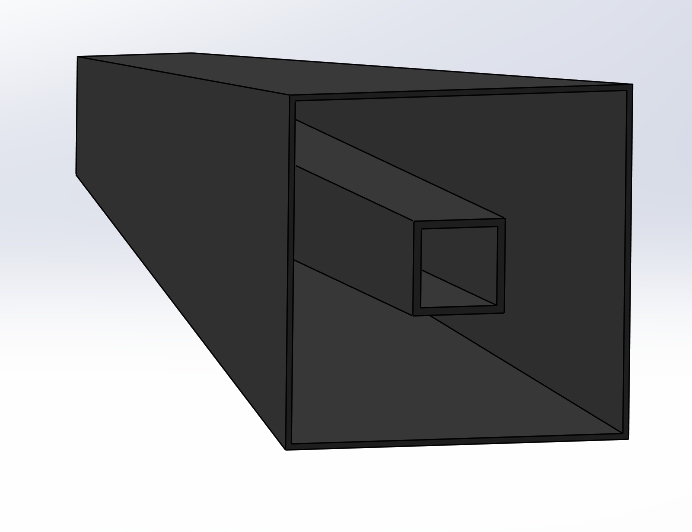
\includegraphics[width=\textwidth]{tail-mount-one}
        \caption{}
        \label{fig:tail-mount-progression:initial}
    \end{subfigure}
    \hfill
    \begin{subfigure}[b]{0.32\columnwidth}
        \centering
        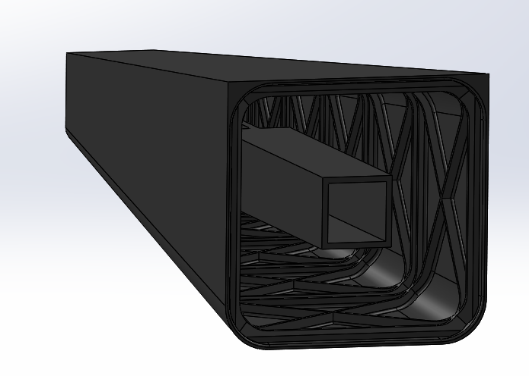
\includegraphics[width=\textwidth]{tail-mount-two}
        \caption{}
        \label{fig:tail-mount-progression:revised}
    \end{subfigure}
    \hfill
    \begin{subfigure}[b]{0.32\columnwidth}
        \centering
        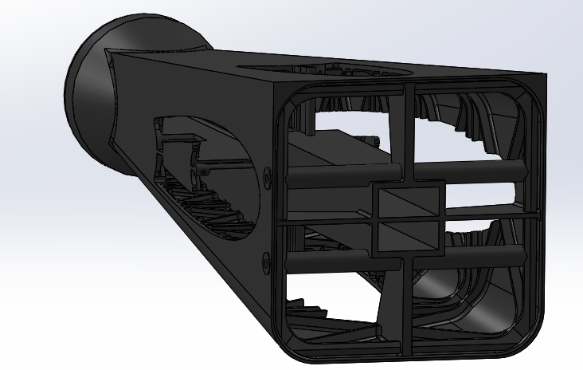
\includegraphics[width=\textwidth]{tail-mount-three}
        \caption{}
        \label{fig:tail-mount-progression:final}
    \end{subfigure}
    
    \caption{progressive iterations of the tail mount design.}
    \label{fig:tail-mount-progression}
\end{figure} 

The process began with a tapered section hollowed out to \mm{1.5} wall thickness, and a rectangular tube added for the tail spar.
The inside and outside corners were filleted. 
Next, ribs were added for lightweight structural support, made by a complex series of combined bodies.
Supporting structure was added from the outside walls to meet the spar tube in the centre.
A mounting location was added for the tail motor, and channels to run securing bolts through were added, as it was intended to make the part in two halves to aid assembly.  
In an assembly, the tail lifting surfaces were added, and moved to the correct position using mates, and then their bodies were subtracted from the mount body. 

Servo mounts were added and a motor mounting solution added based on a teammates previous design, and then a shroud was added over the motor, as well as a wire route for the motor connections.
The structure was eventually split in half and holes for spars added, and the model tidied up for 3D printing. 
A small structure was added to the front to allow for mounting to the foam ahead of it.

Finally, a small 3D printed part was designed to fit into the attachment location at the rear of the tail mount.
This was based on a prior design from earlier on in the project's design process, and simply had a cylinder with wide radial teeth protruding from the inside.
The motor mount had the same teeth, and would slide axially in the cylinder through the gaps, and then rotate, the teeth overlapping to prevent the mount from moving.
Small holes cut through both parts of the mount allowed for threaded inserts to be placed inside, and then screws through the same holes would secure the mount in place. 

% \importimage{tail-mount-slice}{a view of one half of the final tail mount.}{Tail mount slice}{0.4}
% \importimage{tail-mount-final}{a view of the final tail mount design.}{Tail mount design}{0.4}

\begin{figure}[H]
    \centering
    \begin{subfigure}[b]{0.49\columnwidth}
        \centering
        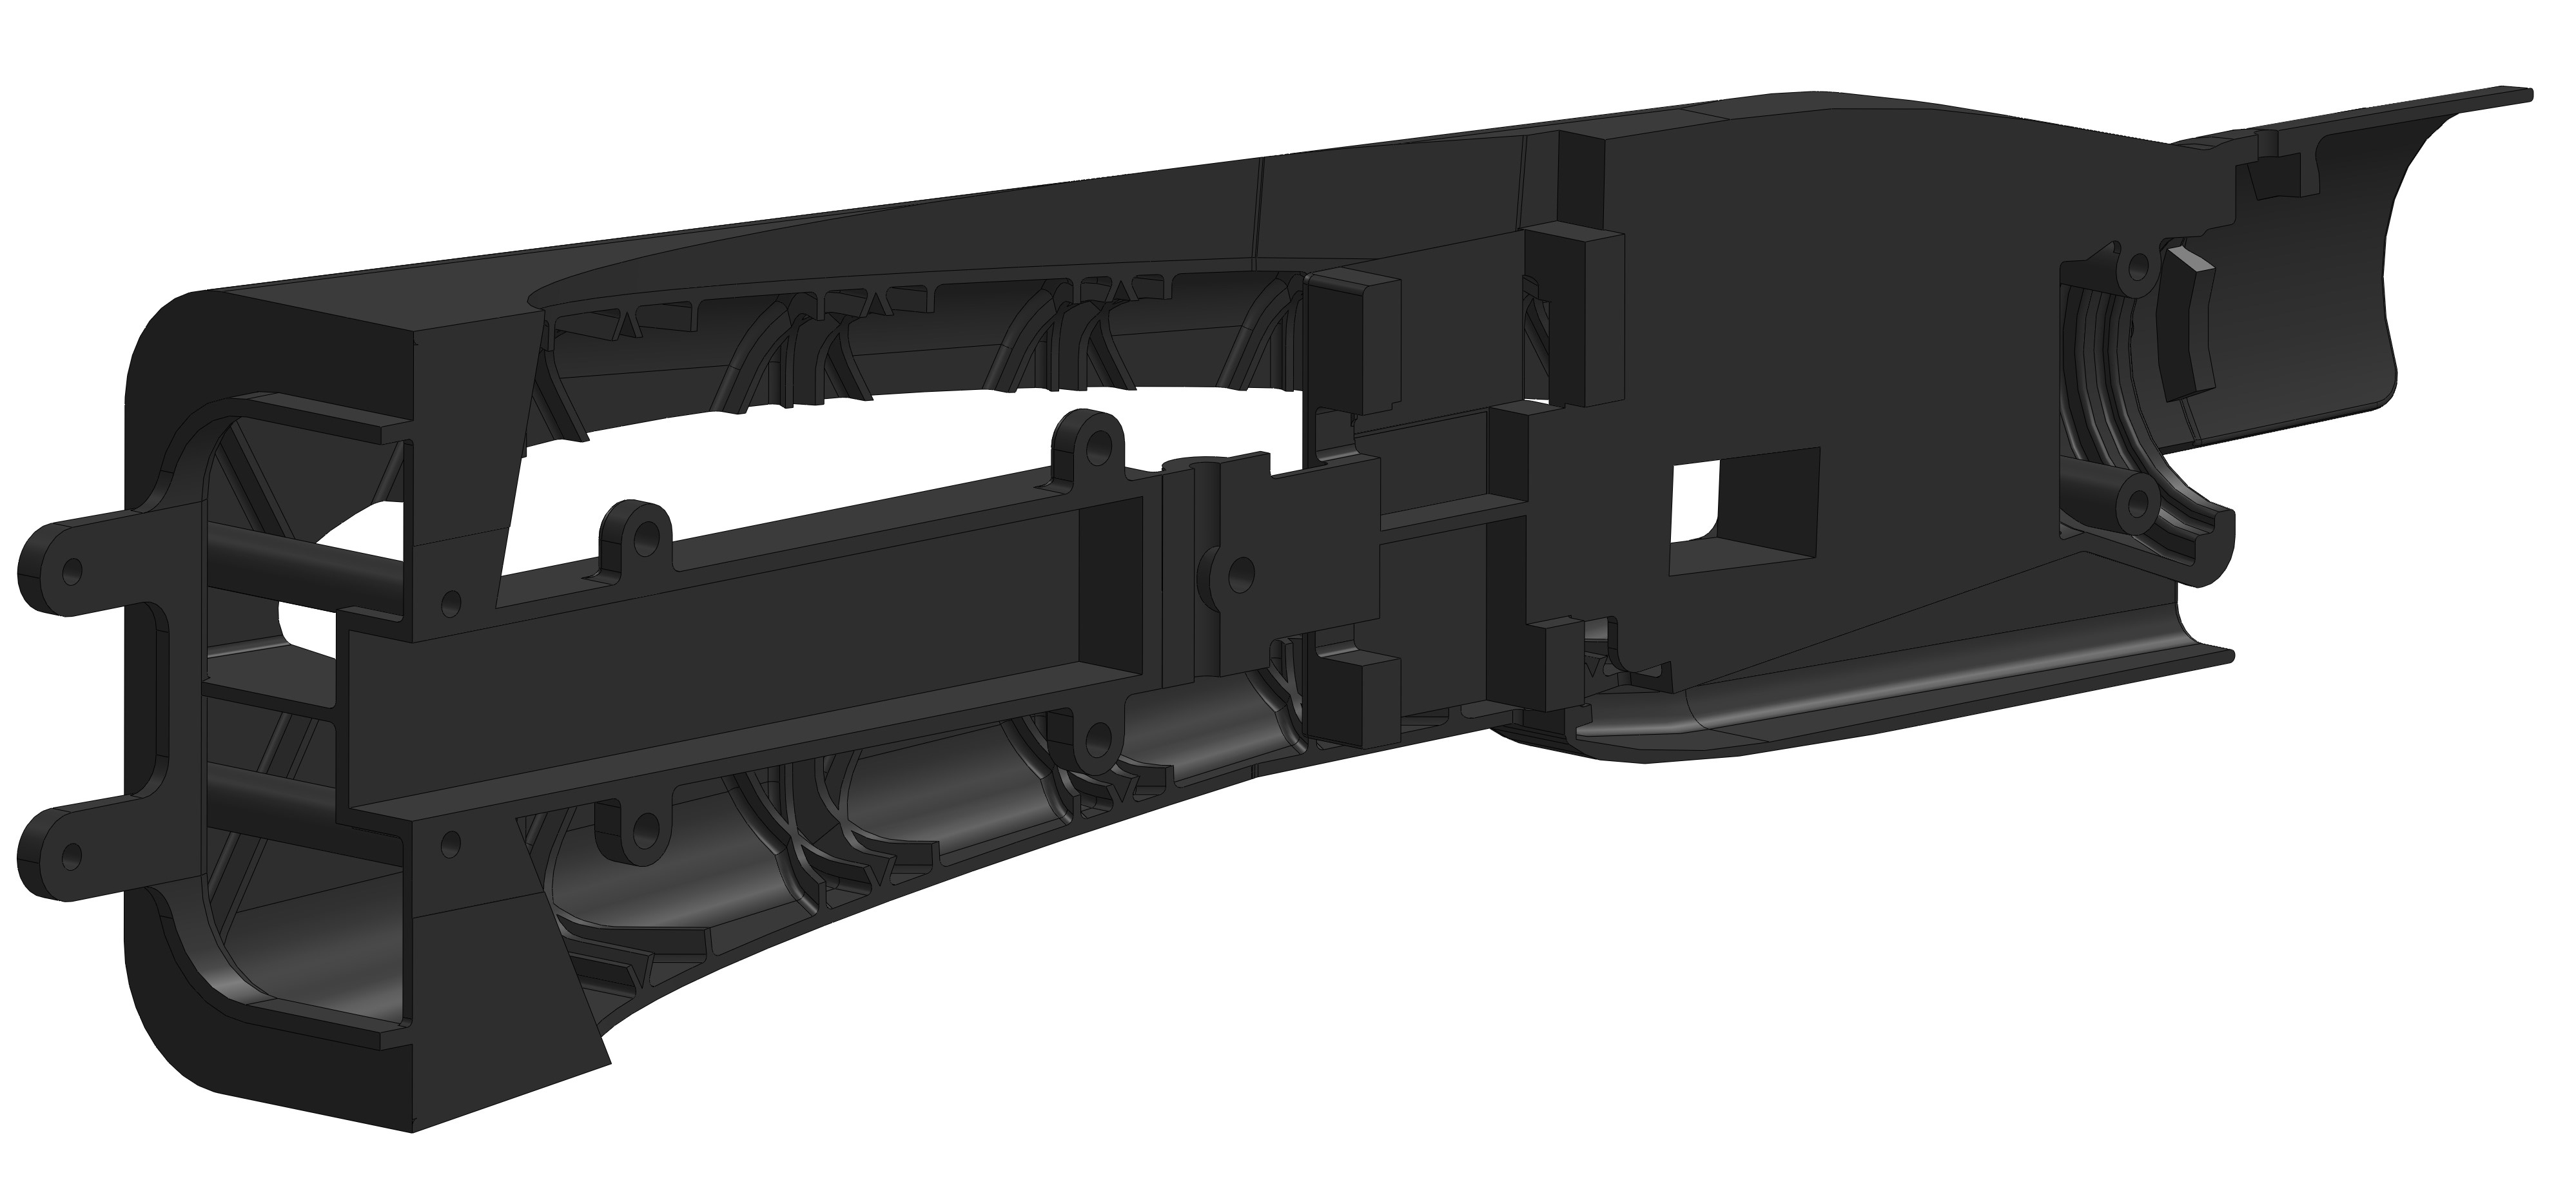
\includegraphics[width=\textwidth]{tail-mount-slice}
        \caption{}
        \label{fig:tail-mount-design:slice}
    \end{subfigure}
    \hfill
    \begin{subfigure}[b]{0.49\columnwidth}
        \centering
        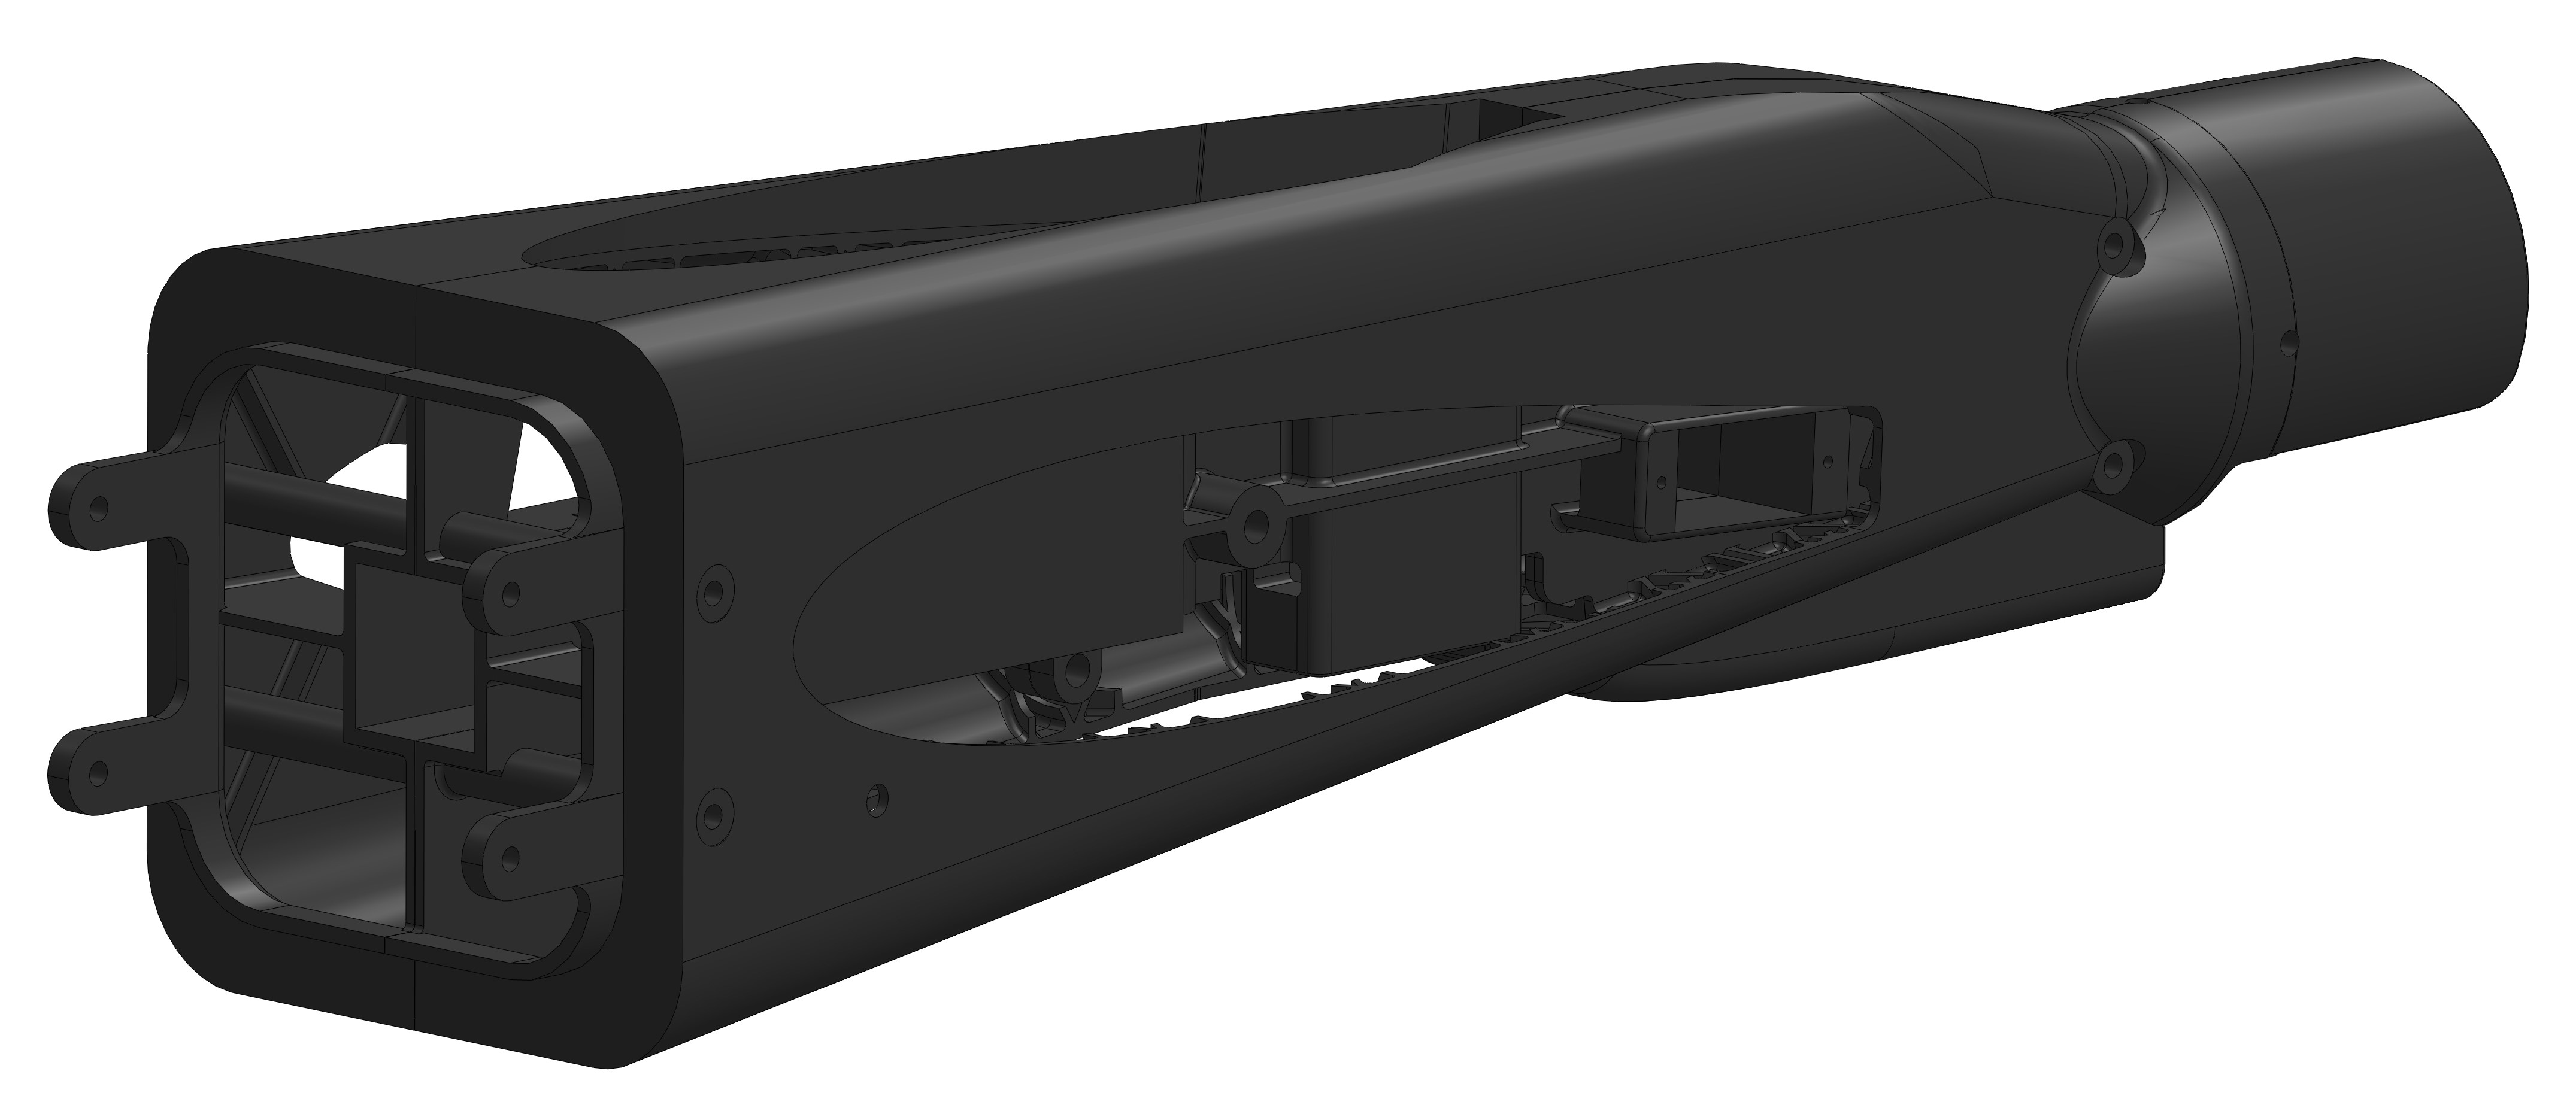
\includegraphics[width=\textwidth]{tail-mount-final}
        \caption{}
        \label{fig:tail-mount-design:whole}
    \end{subfigure}
    
    \caption{final tail mount design; (a) shows a cut view.}
    \label{fig:tail-mount-design}
\end{figure} 

\importimage{exploded-tail}{exploded view of the tail assembly, including fasteners.}{Exploded tail assembly}{0.7}

% TODO: describe final control surface design here?

\section{Avionics} \label{sec:final-design-proposal:avionics}

Few drastic changes were made to the avionics between the revised and final designs.
The final wiring diagram, including all components comprising the avionics and electronics subsystem for the final model, is shown in Figure \ref{fig:wiring-diagram}.

\importimage{wiring-diagram}{wiring diagram for the avionics subsystem.}{Wiring diagram}{0.9}

One key difference not mentioned previously is the inclusion of several signal splitters, designed to split signals for each control surface from the single corresponding output on the flight controller to the multiple servos belonging to that group.
The arrangement of splitters, shown in Figure \ref{fig:signal-splitters}, distributes the signals to the relevant locations while using a minimal amount of wiring and also keeping the number of splitters as low as possible.
Primarily this is accomplished by sharing common lines such as power and ground between groups, and branching individual lines off to servos in a tree-like structure.
In locations where two servos are within a relatively short distance of each other, these are both served by a single splitter, with wires leading to each one.

The splitters themselves (Figure \ref{fig:splitter-schematic}) consist of a copper stripboard with header pins soldered across.
Each spitter is specified in terms of the signals designated as inputs and outputs, and soldering the header pins across the stripboard enables the same signal $-$ from one input $-$ to be output to multiple locations.
Splitters are also chained together where needed, and some splitters have breaks in the stripboard to accommodate a more compact design.
A small outcrop of stripboard is left around the edge of each splitter so that they can be secured in place within the aircraft; it is thought that wires are less likely to become damaged if their attachment points cannot move, thereby reducing the risk of failure or electrical damage.

\importimage{splitter-schematic}{manufacturing schematic for splitter 3; strips are aligned horizontally, with header pins denoted by rectangles and solder denoted by ovals.}{Manufacturing schematic}{0.5}

Ultimately all of the servos $-$ along with the avionics $-$ are powered by the avionics battery via the flight controller.
Jumper wires are soldered to the flight controller, which can plug into the female JST connector that powers the battery.
The battery itself is attached to the electronics tray by velcro, and can therefore be removed with ease.

Along with the flight controller, battery, and receiver, a microcontroller is included for data logging.
The efficiency of the UAV is to be measured by repeatedly sampling the current draw (which can be read through the flight controller's UART port) and multiplying the draw by the time step to sum to a cumulative capacity drawn.
Maintaining this as a cumulative total means it can easily be stored in RAM and downloaded to a computer when the UAV touches down via a serial port.
Because of the miniscule processing requirement of this task and its small size, an Arduino Nano is recommended as the microcontroller of choice.

\begin{figure}[H]
    \centering
    \begin{subfigure}[b]{0.49\columnwidth}
        \centering
        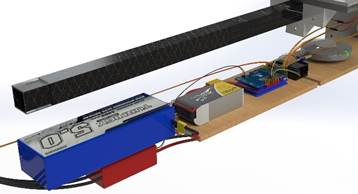
\includegraphics[width=\textwidth]{electronics-housing}
        \caption{Housing bay}
        \label{fig:electronics-subsystem:bay}
    \end{subfigure}
    \hfill
    \begin{subfigure}[b]{0.49\columnwidth}
        \centering
        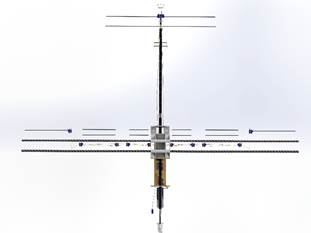
\includegraphics[width=\textwidth]{electronics-exploded}
        \caption{Subsystem, exploded}
        \label{fig:electronics-subsystem:exploded}
    \end{subfigure}
    
    \caption{renders of the key parts of the electronics subsystem.}
    \label{fig:electronics-subsystem}
\end{figure} 

The majority of the electronics subsystem is housed inside a removable electronics bay within the fuselage (Figure \ref{fig:electronics-subsystem}).
Each component of the subsystem was chosen in part for its sleek profile, which means the tray can be removed by sliding it out; this allows quick and easy access to the microcontroller $-$ for data retrieval $-$ and the avionics battery $-$ for recharging $-$ between runs.
In principle, data can be downloaded from the microcontroller and the avionics battery can be swapped out in less time than it takes to swap the PUCs, thereby ensuring that the avionics is not the throttling factor for the effectiveness of the UAV's modularity.

\section{Propulsion} \label{sec:final-design-proposal:propulsion}

% TODO: rewrite in the present tense, more descriptive?

The design of the housing for the motors and its subsidiary systems focused on permitting the repositioning of these system in a small time window without the need for alteration to the design, thereby increasing the number of flights that can be completed in one day.
This was crucial so that the difference in atmospheric conditions are reduced to minimum. 
The use of the PUC design allowed the reduction of wires running through the wing as well as making those components more accessible for maintenance.
Furthermore, the use of a compact design allowed for a standard PUC which could be used in all wing propulsion configurations.
This was achieved by creating a standard simple profile for the surfaces normal to the attachment points; this is evident in Figure \ref{fig:puc-assemblies}.
In order to guarantee a smooth passage of the flow around the housing an adapter is created for each configuration.
This slots onto the standardized surfaces of the power unit cell and mounts directly on the wing surfaces blending the two together.
Furthermore, they ensure that the thrust line in unvaried between tractor and pusher configurations. 

% \importimage{puc-tractor}{PUC section view in top-tractor configuration.}{PUC top tractor}{0.5}
% \importimage{puc-pusher}{PUC section view in top-pusher configuration; yellow is the adaptor, green is the ESC, red is the battery, and blue is the motor.}{PUC top pusher}{0.5}

\begin{figure}[H]
    \centering
    \begin{subfigure}[b]{0.49\columnwidth}
        \centering
        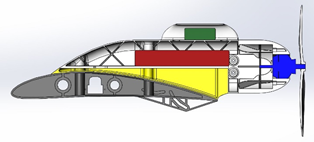
\includegraphics[width=\textwidth]{puc-pusher}
        \caption{Overwing pusher}
        \label{fig:puc-assemblies:pusher}
    \end{subfigure}
    \hfill
    \begin{subfigure}[b]{0.49\columnwidth}
        \centering
        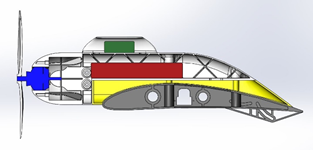
\includegraphics[width=\textwidth]{puc-tractor}
        \caption{Overwing tractor}
        \label{fig:puc-assemblies:tractor}
    \end{subfigure}

    \begin{subfigure}[b]{0.7\columnwidth}
        \centering
        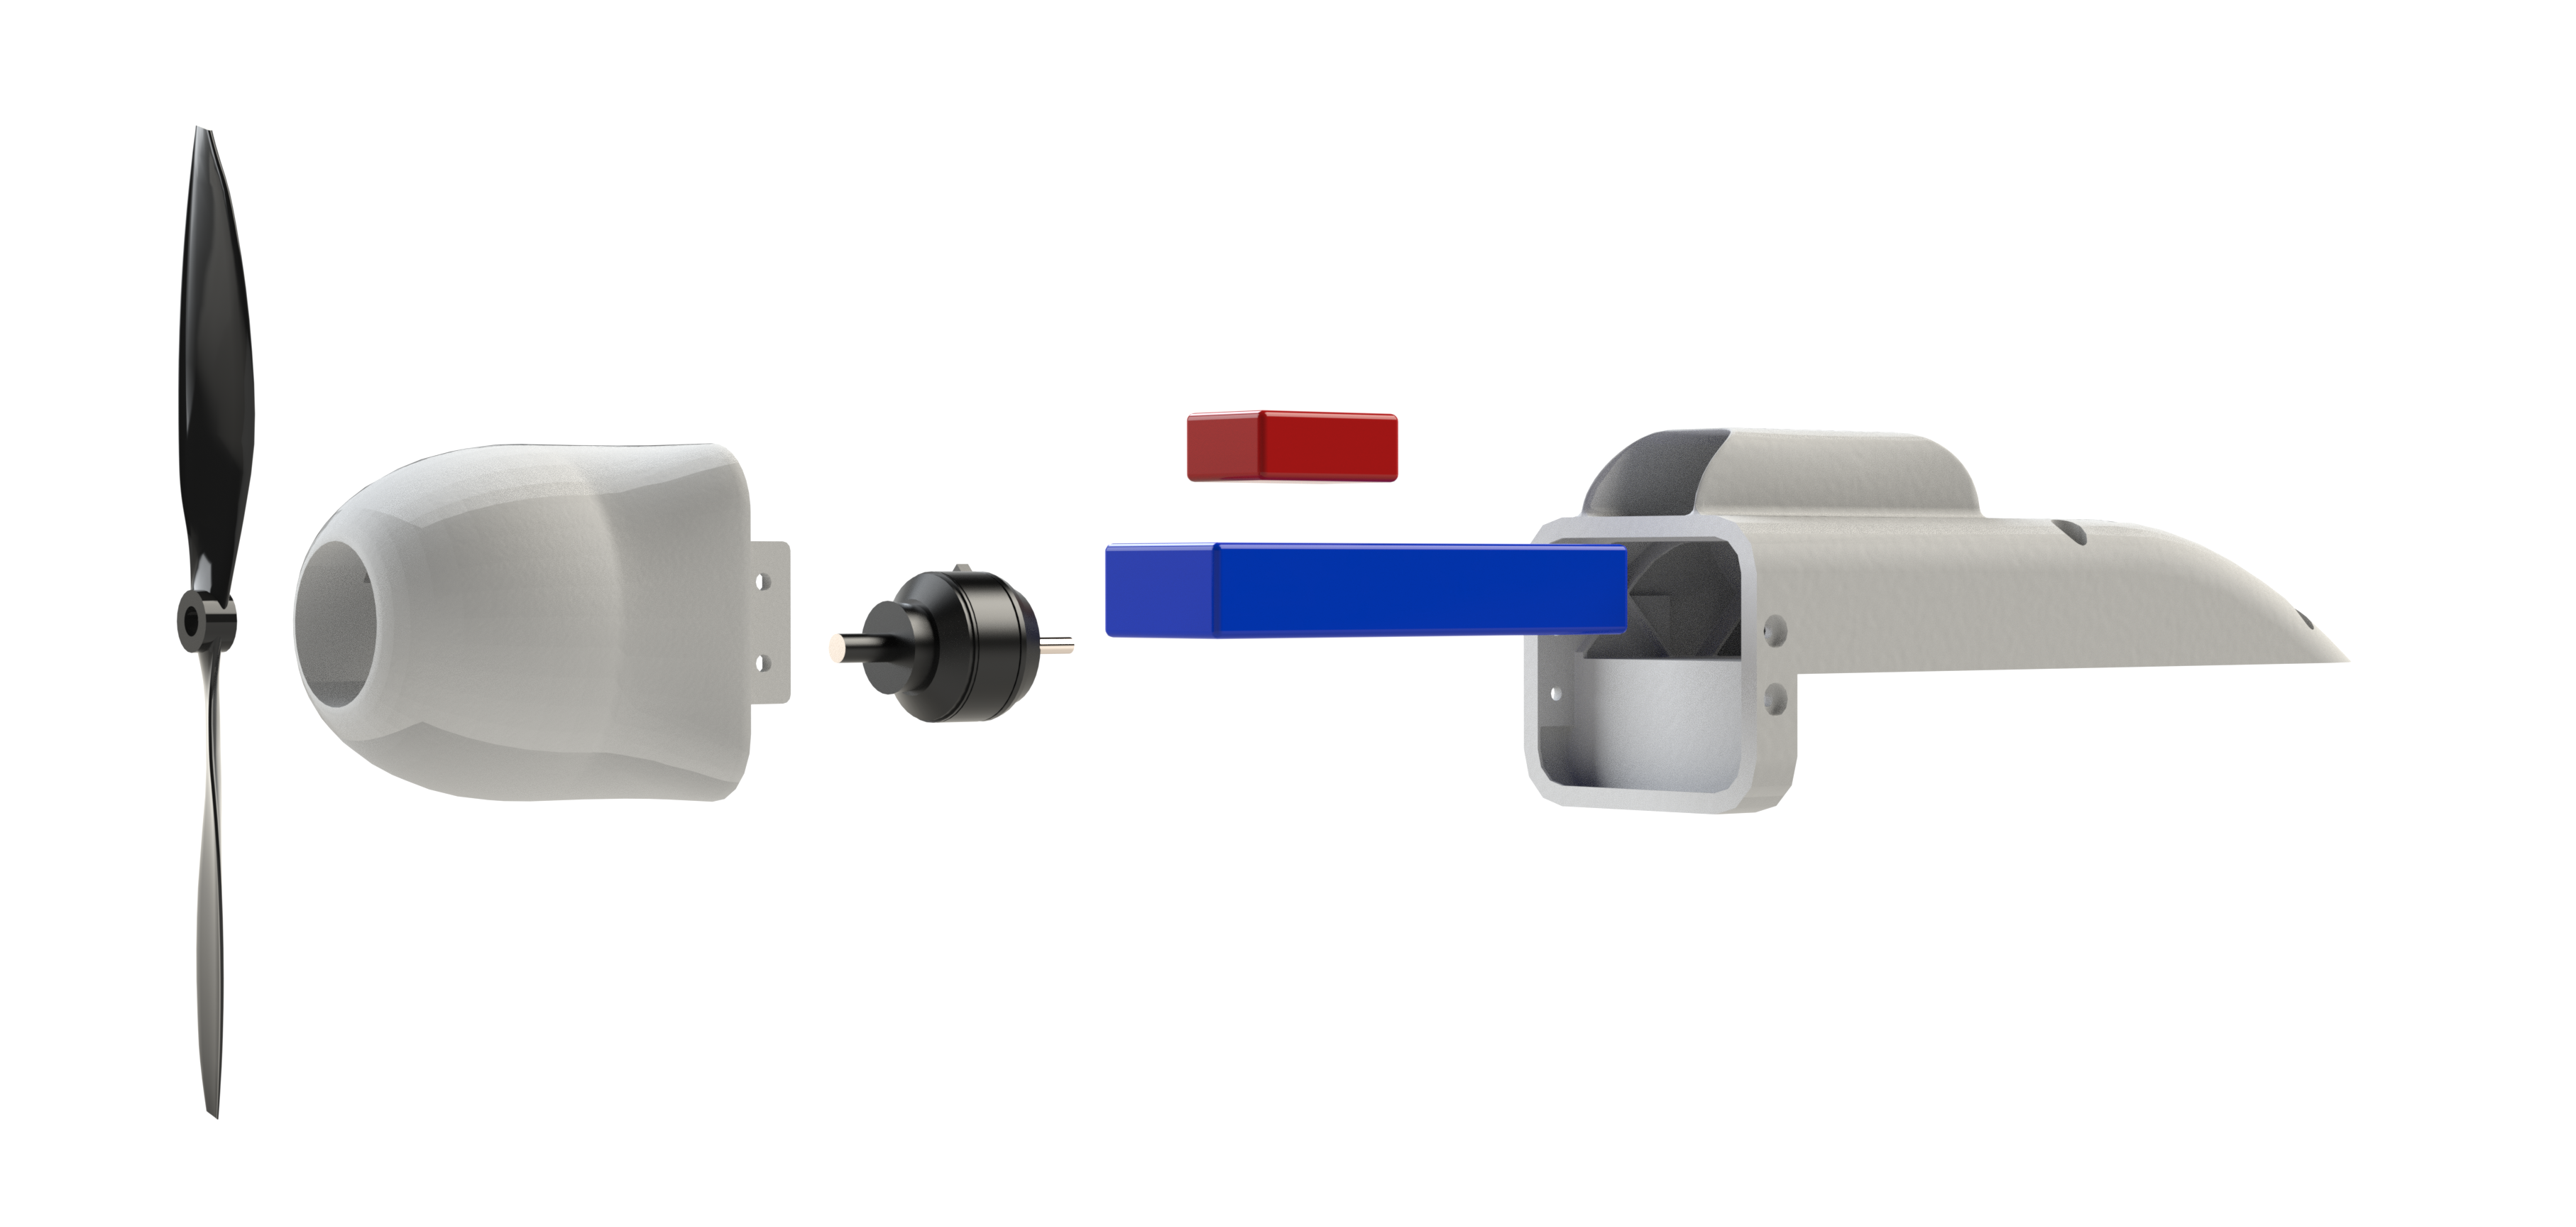
\includegraphics[width=\textwidth]{puc-exploded}
        \caption{Exploded}
        \label{fig:puc-assemblies:exploded}
    \end{subfigure}
    
    \caption{
        various views of the PUC assembly.
        Adapters are in yellow; ESCs are in green; batteries are in red; and motors are in blue.
    }
    \label{fig:puc-assemblies}
\end{figure} 

The distance from the trailing edge to the propeller in the pusher layout is equivalent to the distance from the leading edge to the propeller in the tractor layout.
Moreover, as in can be seen in Figure \ref{fig:puc-assemblies}, the attachment holes for the mounting bolts remain in the same position despite the change in arrangement, thereby allowing propulsion layouts to be changed without modifying the components. 
The power unit cells are also split in two components: a front section and a rear section, permitting to access the components stored inside with the removal of the four M4 bolts securing the two halves together.
Four threaded inserts imbedded in the nylon structure of the front section allow the fitting of the motor.
The battery and the ESC are instead slotted into the rear section of the cell.
The open section into which the ESC is placed ensures the cooling of this component in all configurations setup, avoiding common reliability issues caused by overheated ESCs.
An exploded view of the PUC assembly is shown in Figure \ref{fig:puc-assemblies:exploded}. 

% \importimage{puc-exploded}{exploded view of the PUC assembly.}{Exploded PUC}{0.6}

Due to the fitting of the battery and the ESC, the PUC assembly has a significant weight.
In fact, the CG of the UAV is subject to a noticeable shift as the motor configuration is changed from tractor to pusher.
A reduction in this effect leads to a less significant need to rely on a ballast to maintain the CG in the same location. 
In order to alleviate this effect, the battery was located closer to half chord length with some compromises made for the aerodynamic aspect.
Further lightweighting work produced more efficient components through the use of ribs and reinforcements, where loads concentrate, and thin walls as shown in Figure \ref{fig:puc-design:rear}.
This resulted into an overall housing dry weight of 207 g. 

% \importimage{puc-front}{PUC front section inner structure.}{PUC front section}{0.3}
% \importimage{puc-rear}{PUC rear section inner structure.}{PUC rear section}{0.3}

\begin{figure}[H]
    \centering
    \begin{subfigure}[b]{0.4\columnwidth}
        \centering
        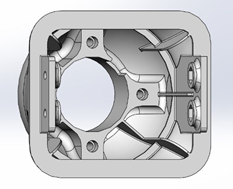
\includegraphics[width=\textwidth]{puc-front}
        \caption{Front}
        \label{fig:puc-design:front}
    \end{subfigure}
    \hfill
    \begin{subfigure}[b]{0.4\columnwidth}
        \centering
        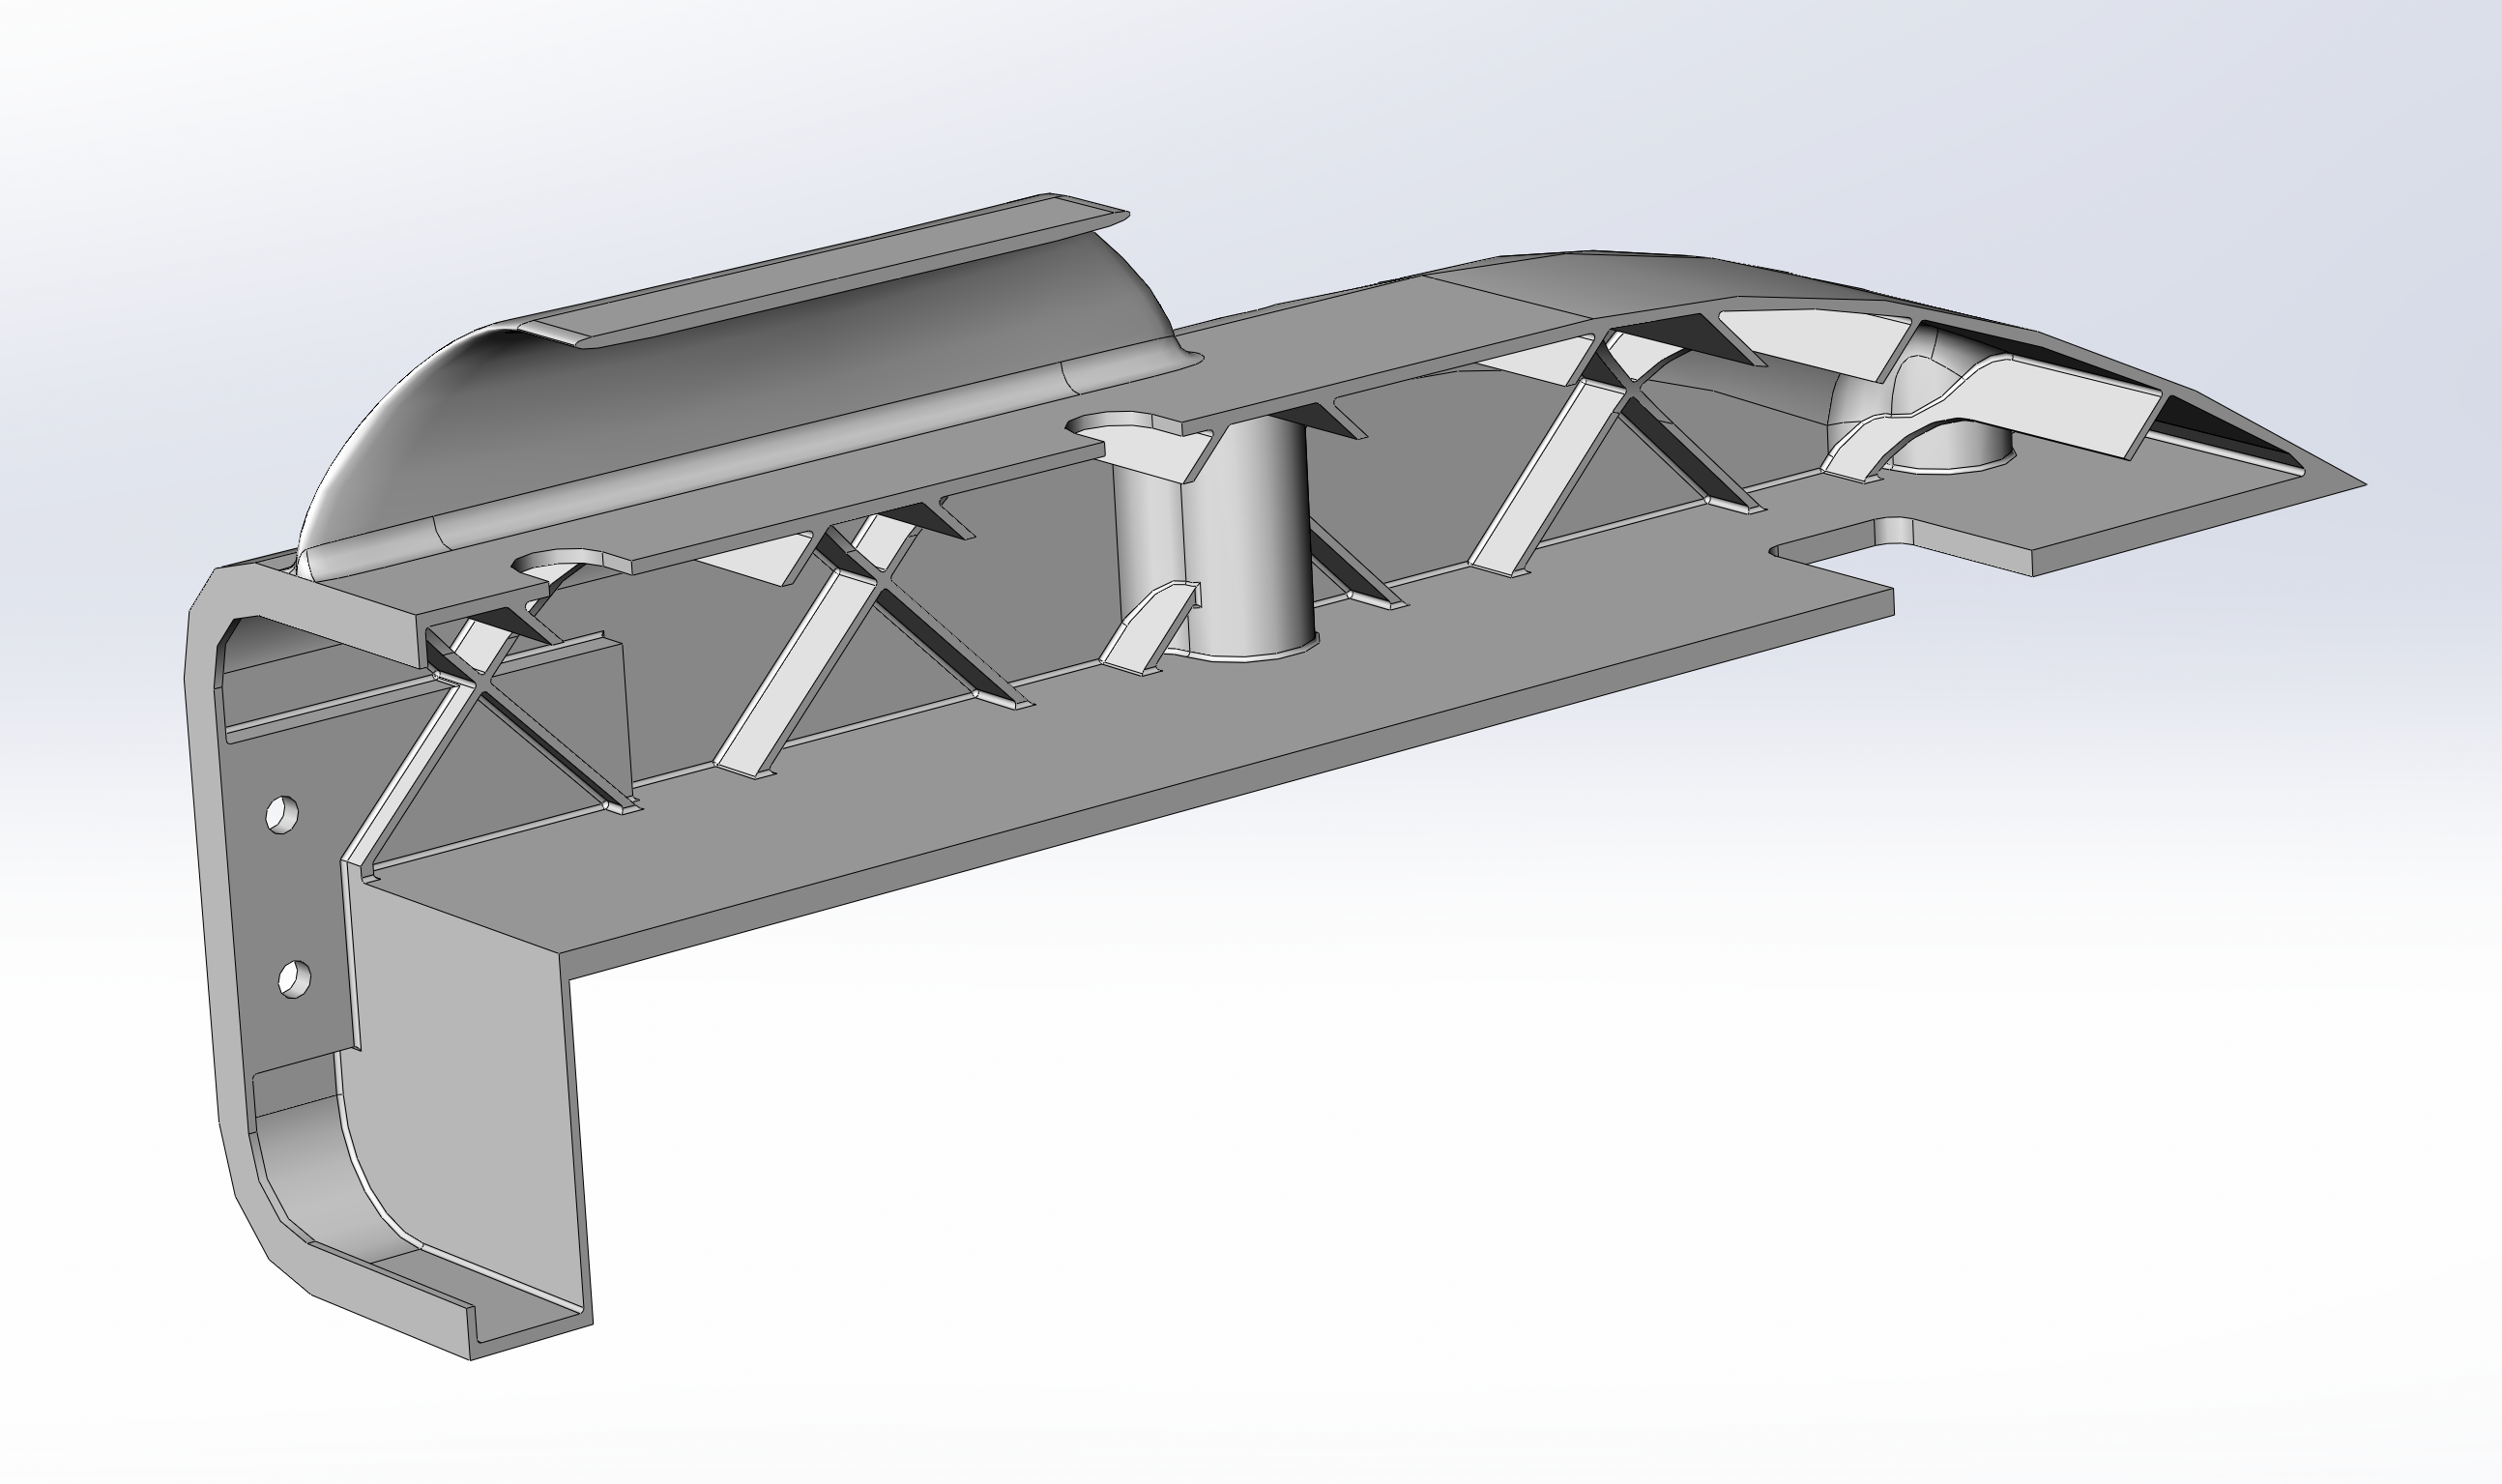
\includegraphics[width=\textwidth]{puc-rear}
        \caption{Rear}
        \label{fig:puc-design:rear}
    \end{subfigure}
    
    \caption{inner structure of the PUC.}
    \label{fig:puc-design}
\end{figure}

\section{Control of variables} \label{sec:final-design-proposal:control-of-variables}

Assessment of the influence of different power unit layouts upon efficiency involves a great many variables, especially when the test is carried on the same vehicle.
Each configuration requires different specifications in order to be mounted and affects the behaviour of the aircraft in different ways.
A pusher mounted motor, for example, will have the tendency to increase wing twist due to the additional weight on the trailing edge of the wing.
Furthermore, for the cases of a tail or nose mounted unit, the tail surfaces will be influenced since they are positioned in the flow field of the propeller.
These are all factors that have a potential influence on the UAV's efficiency.
Hence, in order to have entirely accurate estimates of the influence of solely the propulsion location on performance, multiple vehicles would have to be designed, each one exploiting the advantages of each configuration. 

Due to the time and budget constraints, only one UAV could be built for this project, and as such was the main driving factor behind a simple design which could accommodate all the possible layouts for fair testing at the expense of overall efficiency.
A focus was maintained on obtaining a neutral platform characterised by a constant weight and centre of gravity.
Any increase in cross sectional area caused by mounting structures or aerodynamic effect was considered to be part of the influences induced by the power unit layouts and so was not tightly controlled, but was kept broadly similar. 

% TODO: put this in somewhere
% Due to the outbreak of COVID-19 the flight tests were not able to be carried out as planned, causing the absence of the data necessary to compare the effects of each propulsion layout on the UAV performance.
% In spite of this, throughout the design and development of ELMO UAV, the impact of each propulsion configuration on the aircraft design was assessed.
% The final model does not represent the optimal design for efficiency instead, perhaps, is the conjuncture of all the compromises demanded to ensure the airworthiness of the UAV when flown in any layout. 

As aforementioned, the PUC locations have great influence over the centre of gravity position as well as the overall weight.
The configurations which offer the lightest model are the fuselage mounted power units.
These do not require additional additively manufactured components for motor, battery and ESC housing since the housings are integrated into the nose and tail designs.
Thanks to the positioning of the battery and ESC in the front section of the fuselage, the nose mounted power unit layout presents a positive influence over the CG position by moving it forward to \pc{40} chord length.
Such a positive effect is reduced when, for the same battery and ESC position, the motor is located on the tail.
This results in a shift in CG to \pc{60} chord length.
The main difference exhibited between tractor and pusher configurations is also a shift in the centre of gravity.
This results in its moving backwards for a pusher configuration with respect to its position at \pc{53} chord in the case of a tractor configuration.

A single engine layout, although lighter, demands more reliable components due to the absence of a second propulsion unit in case of engine failure.
Furthermore, for the case of a tail mounted motor, there is the risk of the propeller striking the runway during takeoff or landing.
The addition of a lower vertical stabiliser equipped with a tip bumper protects the propeller in the event of a tail strike. 

For any wing layout, additional PUCs must be mounted.
In addition to this, the use of two power units leads to a larger increase in weight as compared to a single motor configuration.
The propulsion unit position also influences the design of the wing structure.
The bending moment induced by the wing motor configuration closest to the fuselage is much smaller in magnitude than the tip configuration, mandating a stiffer wing structure despite being heavier.

In spite of the numerous design features required to accommodate the modularity of the UAV $-$ while maintaining consistency in key variables to ensure the validity of experiments by isolating the effect of the position of the propulsion system $-$ the final model's total mass remains below the \kg{7} threshold originally set.

\end{document}
